\input{../lib.tex}

\usepackage{verbatim} % for comment

\usepackage[framemethod=tikz]{mdframed}
%\usepackage{tikzpagenodes}
\usepackage{hyperref} %Allows to make references (\ref{}), pdf links are now clickable.
\usetikzlibrary{calc, arrows}

% greyarrow has much better handling of page breaks, see the link on stackoverflow for more info
\def\SolStyle{greyarrow}
\ifthenelse{\isundefined{\SolStyle}}{\def\SolStyle{greyarrow}}{}
\ifthenelse{\equal{\SolStyle}{greyarrow}}
{
  %http://tex.stackexchange.com/questions/50877/excursus-environment-using-mdframed-issue-with-page-breaks
\tikzset{
   excursus arrow/.style={%
    line width=2pt,
    draw=gray!40,
    rounded corners=2ex,
   },
   excursus head/.style={
    fill=white,
    font=\bfseries\sffamily,
    text=gray!80,
    anchor=base west,
   },
}

\mdfdefinestyle{mysquare}{%
  singleextra={%
   \path let \p1=(P), \p2=(O) in (\x2,\y1) coordinate (Q);%
   \path let \p1=(Q), \p2=(O) in (\x1,{(\y1-\y2)/2}) coordinate (M);%
   \path [excursus arrow, round cap-to]%
   ($(O)+(5em,0ex)$) -| (M) |- %
   ($(Q)+(12em,0ex)$) .. controls +(0:16em) and +(185:6em) .. %
   ++(23em,2ex);%
   \node [excursus head] at ($(Q)+(2.5em,-0.75pt)$) {Solution};},
  firstextra={%
   \path let \p1=(P), \p2=(O) in (\x2,\y1) coordinate (Q);
   \path [excursus arrow,-to]
   (O) |- %
   ($(Q)+(12em,0ex)$) .. controls +(0:16em) and +(185:6em) .. %
    ++(23em,2ex);
   \node [excursus head] at ($(Q)+(2.5em,-2pt)$) {Solution};
  },
  secondextra={%
   \path let \p1=(P), \p2=(O) in (\x2,\y1) coordinate (Q);
   \path [excursus arrow,round cap-]
   ($(O)+(5em,0ex)$) -| (Q);
  },
  middleextra={%
   \path let \p1=(P), \p2=(O) in (\x2,\y1) coordinate (Q);
   \path [excursus arrow](O) -- (Q);
 },
 middlelinewidth=2.5em,middlelinecolor=white,
 hidealllines=true,topline=true,
 innertopmargin=0.5ex,
 innerbottommargin=2.5ex,
 innerrightmargin=2pt,
 innerleftmargin=2ex,
 skipabove=0.87\baselineskip,
 skipbelow=0.62\baselineskip,
}

}
{
  %http://tex.stackexchange.com/questions/107191/indented-box-that-split-in-multiple-pages
\mdfdefinestyle{mysquare}{%
  leftmargin=0pt,
  rightmargin={\dimexpr4pt+2ex\relax},
  innertopmargin=2\baselineskip,
  skipabove={\dimexpr0.5\baselineskip+\topskip\relax},
  skipbelow={\dimexpr0.5\baselineskip+\topskip\relax},
  singleextra={% Single extra applies when it fits in a single page
  \path let \p1=(P), \p2=(O)
    in node[font=\bfseries] at ([yshift=-2ex]0.5*\x1-\x2,\y1) {Solution};
  \fill[black] ([xshift=2pt,yshift=2pt]P) rectangle ++(1ex,1ex);
  \fill[black] ([xshift=-2pt,yshift=-2pt]O) rectangle ++(-1ex,-1ex);
  \fill[black] ([xshift=-2pt,yshift=2pt]O|-P) rectangle ++(-1ex,1ex);
  \fill[black] ([xshift=2pt,yshift=-2pt]O-|P) rectangle ++(1ex,-1ex);
  },
  firstextra={% First extra applies on the first page when it doesn't fit in one page
  \path let \p1=(P), \p2=(O)
    in node[font=\bfseries] at ([yshift=-2ex]0.5*\x1-\x2,\y1) {Solution};
  \fill[fill=black] ([xshift=2pt,yshift=2pt]P) rectangle ++(1ex,1ex);
  \fill[black] ([xshift=-2pt,yshift=2pt]O|-P) rectangle ++(-1ex,1ex);
  },
  secondextra={% First extra applies on the last page when it doesn't fit in one page
  \fill[fill=black] ([xshift=2pt,yshift=-2pt]O-|P) rectangle ++(1ex,-1ex);
  \fill[black] ([xshift=-2pt,yshift=-2pt]O) rectangle ++(-1ex,-1ex);
  }
}

}


\ifthenelse{\isundefined{\Sol}}{\def\Sol{true}}{}
\ifthenelse{\equal{\Sol}{false}}
{
  \newenvironment{solution}{\expandafter\comment}{\expandafter\endcomment}
}
{
  \newmdenv[style=mysquare]{solution}
}

\newcommand{\nosolution}
{Cet exercice ne contient pas encore de solution.
Vous êtes invité à nous en soumettre une à l'adresse suivante
\begin{center}
\url{https://github.com/blegat/LINMA1691}
\end{center}
ou par mail.}

\parindent0mm

\setlength{\textwidth}{15cm}
\setlength{\oddsidemargin}{0.50cm}
\setlength{\textheight}{8.7in}
\setlength{\topmargin}{-0.5in}

\newcommand{\R}{{\mbox{\bf R}}}

\title{INMA1691 - Théorie et Algorithmique des Graphes : Exercices}
\input{../authors.tex}

\begin{document}
%%%%%%%%%%%%%%%%%%%%%%%%%%%%%%%%%%%%%%%%%%%%%%%%%%%%%%%%%%%%%%%
%%%%%%%%%%%%%%%%%%%%%%%% PAGE DE GARDE %%%%%%%%%%%%%%%%%%%%%%%%
%%%%%%%%%%%%%%%%%%%%%%%%%%%%%%%%%%%%%%%%%%%%%%%%%%%%%%%%%%%%%%%
\pagenumbering{gobble}% Remove page numbers
\maketitle
\begin{center}
  \textit{Basé sur les séances de TP données par
  Adeline Decuyper et Romain Hollanders}\\
  \includegraphics[width=100pt]{../img/logo}\\
  \textbf{Code source et bug tracker}\\
  \url{https://github.com/blegat/LINMA1691}
\end{center}
\newpage
\clearpage

%%%%%%%%%%%%%%%%%%%%%%%%%%%%%%%%%%%%%%%%%%%%%%%%%%%%%%%%%%%%%%%
%%%%%%%%%%%%%%%%%%%%%%% Table Of Contents %%%%%%%%%%%%%%%%%%%%%
%%%%%%%%%%%%%%%%%%%%%%%%%%%%%%%%%%%%%%%%%%%%%%%%%%%%%%%%%%%%%%%
\pagenumbering{arabic}% Arabic page numbers (and reset to 1)
\tableofcontents

\section{Graphes connexes, eulériens et bipartis }
\subsection{Graphes}

\index{graphe}
\begin{mydef}
  \label{def:graph}
  Un \emph{graphe} est un triplet ($V$, $E$, $\varphi$), où :
  \begin{itemize}
    \item $V$ est un ensemble dont les éléments sont appelés sommets ou noeuds;
    \item $E$ est un ensemble dont les éléments sont appelés arêtes;
    \item $\varphi$ est une fonction, dîte fonction d'incidence, qui associe à chaque arête un sommet ou une \emph{paire} de sommets.
  \end{itemize}
\end{mydef}

\index{sommets adjacents}
\begin{mydef}
  Deux sommets incidents à la même arête sont dits \emph{adjacents}.
\end{mydef}

\index{boucle}
\begin{mydef}
  Une arête incidente à un seul sommet est une \emph{boucle}.
\end{mydef}

\index{degré}
\begin{mydef}
  Le \emph{degré} d'un sommet est le nombre d'arêtes incidentes à celui-ci.
\end{mydef}

\index{graphe!sous-graphe}
\begin{mydef}

  Un \emph{sous-graphe du graphe} ($V$, $E$, $\varphi$) est un graphe ($V'$, $E'$, $\varphi'$) avec :
  \begin{itemize}
    \item $V' \subseteq V$ ;
    \item $E' \subseteq E$ ;
    \item $\varphi'$ est la restriction de $\varphi$ à $E'$.
  \end{itemize}

\end{mydef}

\index{isomorphisme}
\subsection{Isomorphisme de Graphes}
\begin{mydef}
  Deux graphes ($V$, $E$, $\varphi$) et ($V'$, $E'$, $\varphi'$) sont dits \emph{isomorphes} s'il existe des bijections $f:V \to V'$ et $g:E \to E'$ telles que :
  \begin{center}
    $\varphi(e) = \{u, v\}$ ssi $\varphi(g(e)) = \{f(u), f(v)\}$.
  \end{center}
  Deux graphes sont isomorphes s'il y a une bijection entre les noeuds et les arêtes.
\end{mydef}

\begin{myexem}
  Voici deux exemples d'isomorphisme du même graphe :
    \begin{figure} [!h]
      \centering
	    \subfigure[]
    	{
    	  \begin{tikzpicture}[scale = 0.75]
          \node[draw, circle] at ( 0, 1.5)  (1) {1};
          \node[draw, circle] at ( 2, 0  )  (2) {2};
          \node[draw, circle] at ( 1,-1.5)  (3) {3};
          \node[draw, circle] at (-1,-1.5)  (4) {4};
          \node[draw, circle] at (-2, 0  )  (5) {5};

          \draw[-] (1) edge [bend left] node[anchor = south] {a} (2);
          \draw[-] (2) edge [bend left] node[anchor = west]  {b} (3);
          \draw[-] (3) edge [bend left] node[anchor = north] {c} (4);
          \draw[-] (4) edge [bend left] node[anchor = east]  {d} (5);
          \draw[-] (5) edge [bend left] node[anchor = east]  {e} (1);
        \end{tikzpicture}
      }
      % Cette ligne de commentaire semble être nécessaire pour que les figures soient affichées sur une ligne
      \subfigure[]
      {
        \begin{tikzpicture}[scale = 0.75]
          \node[draw, circle] at ( 0, 1.5)  (1) {$1'$};
          \node[draw, circle] at ( 2, 0.5)  (2) {$2'$};
          \node[draw, circle] at ( 1,-1.5)  (3) {$3'$};
          \node[draw, circle] at (-1,-1.5)  (4) {$4'$};
          \node[draw, circle] at (-2, 0.5)  (5) {$5'$};

          \draw[-] (1) edge [bend left] node[pos=0.05, anchor = west] {$a'$} (3);
          \draw[-] (2) edge node[anchor = north] {$b'$} (5);
          \draw[-] (2) edge node[pos=0.5, anchor = west] {$c'$} (4);
          \draw[-] (3) edge node[pos=0.5, anchor = east] {$d'$} (5);
          \draw[-] (1) edge [bend right] node[pos=0.05, anchor = east] {$e'$} (4);

        \end{tikzpicture}
      }
      % Cette ligne de commentaire semble être nécessaire pour que les figures soient affichées sur une ligne
      \subfigure[]
      {
        \begin{tikzpicture}[scale = 0.75]
          \node[draw, circle] at ( 0, 1.5)  (1) {$1'$};
          \node[draw, circle] at ( 2, 0  )  (4) {$4'$};
          \node[draw, circle] at ( 1,-1.5)  (2) {$2'$};
          \node[draw, circle] at (-1,-1.5)  (5) {$5'$};
          \node[draw, circle] at (-2, 0  )  (3) {$3'$};

          \draw[-] (1) edge [bend left] node[anchor = south] {$e'$} (4);
          \draw[-] (4) edge [bend left] node[anchor = west]  {$c'$} (2);
          \draw[-] (2) edge [bend left] node[anchor = north] {$b'$} (5);
          \draw[-] (5) edge [bend left] node[anchor = east]  {$d'$} (3);
          \draw[-] (3) edge [bend left] node[anchor = east]  {$a'$} (1);
        \end{tikzpicture}
      }
    \end{figure}
    Notons que les graphes \emph{b} et \emph{c} sont les mêmes, leurs noeuds ont simplement été réordonnés.\\
    L'isomorphisme entre \emph{a} et les deux autres est donné par : \\

    \begin{tabular}{lll}
      $f(1)=1'$ & $g(a)=e'$ \\
      $f(2)=4'$ & $g(b)=c'$ & $\varphi(a) = \{1, 2\}$\\
      $f(3)=2'$ & $g(c)=b'$ & $\varphi'(a') = \{1', 3'\}$\\
      $f(4)=5'$ & $g(d)=d'$ & $\varphi'(g(a)) = \{f(1), f(2)\}$\\
      $f(5)=3'$ & $g(e)=a'$ \\
    \end{tabular}
    \newline
    \newline
    \noindent
    Notons aussi que plusieurs résultats sont possibles :
    \begin{figure}[!h]
      \centering
      \subfigure[]
      {
        \begin{tikzpicture}[scale = 0.75]
          \node[draw, circle] at ( 0, 1.5)  (1) {1};
          \node[draw, circle] at ( 2, 0  )  (2) {2};
          \node[draw, circle] at ( 1,-1.5)  (3) {3};
          \node[draw, circle] at (-1,-1.5)  (4) {4};
          \node[draw, circle] at (-2, 0  )  (5) {5};

          \draw[-] (1) edge [bend left] node[anchor = south] {a} (2);
          \draw[-] (2) edge [bend left] node[anchor = west]  {b} (3);
          \draw[-] (3) edge [bend left] node[anchor = north] {c} (4);
          \draw[-] (4) edge [bend left] node[anchor = east]  {d} (5);
          \draw[-] (5) edge [bend left] node[anchor = east]  {e} (1);
        \end{tikzpicture}
      }
      % Cette ligne de commentaire semble être nécessaire pour que les figures soient affichées sur une ligne
      \subfigure[]
      {
        \begin{tikzpicture}[scale = 0.75]
          \node[draw, circle] at ( 0, 1.5)  (1) {$1'$};
          \node[draw, circle] at ( 2, 0.5)  (2) {$2'$};
          \node[draw, circle] at ( 1,-1.5)  (3) {$3'$};
          \node[draw, circle] at (-1,-1.5)  (4) {$4'$};
          \node[draw, circle] at (-2, 0.5)  (5) {$5'$};

          \draw[-] (1) edge [bend left] node[pos=0.05, anchor = west] {$a'$} (3);
          \draw[-] (2) edge node[anchor = north] {$d'$} (5);
          \draw[-] (2) edge node[pos=0.5, anchor = west] {$c'$} (4);
          \draw[-] (3) edge node[pos=0.5, anchor = east] {$b'$} (5);
          \draw[-] (1) edge [bend right] node[pos=0.05, anchor = east] {$e'$} (4);
        \end{tikzpicture}
      }
      \subfigure[]
      {
        \begin{tikzpicture}[scale = 0.75]
          \node[draw, circle] at ( 0, 1.5)  (1) {$1'$};
          \node[draw, circle] at ( 2, 0  )  (3) {$3'$};
          \node[draw, circle] at ( 1,-1.5)  (5) {$5'$};
          \node[draw, circle] at (-1,-1.5)  (2) {$2'$};
          \node[draw, circle] at (-2, 0  )  (4) {$4'$};

          \draw[-] (1) edge [bend left] node[anchor = south] {$a'$} (3);
          \draw[-] (3) edge [bend left] node[anchor = west]  {$b'$} (5);
          \draw[-] (5) edge [bend left] node[anchor = north] {$d'$} (2);
          \draw[-] (2) edge [bend left] node[anchor = east]  {$c'$} (4);
          \draw[-] (4) edge [bend left] node[anchor = east]  {$e'$} (1);
        \end{tikzpicture}
      }
    \end{figure}

    \begin{tabular}{lll}
      $f(1)=1'$ & $g(a)=a'$ \\
      $f(2)=3'$ & $g(b)=b'$ \\
      $f(3)=5'$ & $g(c)=d'$ \\
      $f(4)=2'$ & $g(d)=c'$ \\
      $f(5)=4'$ & $g(e)=e'$ \\
    \end{tabular}
    \newline
    \newline
    Les six graphes de cet exemple sont isomorphes entre eux.
\end{myexem}

\subsection{Parcours eulérien}
\index{parcours}
\begin{mydef}
  Un \emph{parcours} est fermé si $v_0 = v_n$.
\end{mydef}

\index{chemin}
\begin{mydef}
  Un \emph{chemin} est un parcours dont tous les sommets sont distincts.
\end{mydef}

\index{cycle}
\begin{mydef}
  Un \emph{cycle} est un parcours fermé dont tous les sommets d'origine et intérieurs sont tous distincts.
\end{mydef}

\index{graphe!graphe connexe}
\begin{mydef}
  Un \emph{graphe} est \emph{connexe} si pour chaque pair de points il existe un parcours qui les relie. Les \emph{composantes connexes} d'un graphe sont ses sous-graphes connexes maximaux.
\end{mydef}

\index{parcours!parcours eulérien}
\index{graphe!graphe eulérien}
\begin{mydef}
  Un \emph{parcours} est \emph{eulérien} s'il visite chaque arête une et une seule fois. Un \emph{graphe} est \emph{eulérien} s'il existe un parcours eulérien fermé.
\end{mydef}

\begin{mytheo} [Théorème d'Euler]
  Un graphe connexe est eulérien ssi tous les sommets sont de degré pair.
  \begin{proof}
    \noindent
    \newline
    \fbox{$\Longrightarrow$}
    \newline
    Chaque arête incidente à un noeud $x$ est utilisé par le parcours eulérien:
    \begin{itemize}
      \item soit pour entrer dans $x$;
      \item soit pour en sortir.
    \end{itemize}
    À chaque arête entrante correspond une arête sortante (celle qui suit dans le parcours sauf pour la dernière et la première).\\
    Donc, il y a une bijection entre les arêtes entrantes et les arêtes sortantes.\\
    $\longrightarrow$ degré pair \\

    \noindent
    \fbox{$\Longleftarrow$}
    \newline
    On va construire un parcours eulérien :
    \begin{enumerate}
      \item On part d'un noeud arbitraire $x_0$.
      \item On prend une arête incidente à $x_0$, on arrive à un nouveau noeud.
      \item Par parité, il y a au moins une arête non utilisée, on la prend, etc...
        Quand il n'y a plus d'arête disponible, on est forcément arrivé à $x_0$ car
        pour tout autre noeud $y$, en arrivant à $y$, on a utilisé un nombre impair d'arêtes incidentes à $y$.
    \end{enumerate}
    \begin{center}
      \begin{tikzpicture}[scale = 0.75]
        \node[draw, circle] at (-3, 0  )  (1)  {$x_0$};
        \node[draw, circle] at (-2, 1.5)  (2)  {};
        \node[draw, circle] at (-2,-1.5)  (3)  {};
        \node[draw, circle] at (-1, 0  )  (4)  {};
        \node[draw, circle] at ( 0, 1.5)  (5)  {};
        \node[draw, circle] at ( 0,-1.5)  (6)  {};
        \node[draw, circle] at ( 1, 0  )  (7)  {$x_1$};
        \node[draw, circle] at ( 2, 1.5)  (8)  {};
        \node[draw, circle] at ( 2,-1.5)  (9)  {};
        \node[draw, circle] at ( 3, 0  )  (10) {};

        \draw[-] (1) edge node {} (2);
        \draw[dotted] (1) edge node {} (3);
        \draw[-] (2) edge node {} (4);
        \draw[-] (3) edge node {} (4);
        \draw[-] (4) edge node {} (5);
        \draw[-] (4) edge node {} (6);
        \draw[-] (5) edge node {} (7);
        \draw[-] (6) edge node {} (7);
        \draw[-] (7) edge node {} (8);
        \draw[-] (7) edge node {} (9);
        \draw[-] (8) edge node {} (10);
        \draw[-] (9) edge node {} (10);
      \end{tikzpicture}
    \end{center}
    On a un parcours fermé :
    \begin{itemize}
      \item Si toutes les arêtes incidentes aux $x$ noeuds traversés par ce parcours sont utilisées, alors ce parcours est eulérien;
      \item Sinon, il y a $x_1 \in$ parcours avec au moins une arête non exploitée.
    \end{itemize}
    \begin{center}
      \begin{tikzpicture}[scale = 0.75]
        \node[draw, circle] at (-4, 0  )  (1)  {};
        \node[draw, circle] at (-4,-1.5)  (2)  {};
        \node[draw, circle] at (-2, 0  )  (3)  {$x_0$};
        \node[draw, circle] at (-2,-1.5)  (4)  {};
        \node[draw, circle] at (-2, 1.5)  (5)  {};
        \node[draw, circle] at ( 0, 1.5)  (6)  {};
        \node[draw, circle] at ( 0, 0  )  (7)  {$x_1$};
        \node[draw, circle] at ( 0,-1.5)  (8)  {};
        \node[draw, circle] at ( 2,-1.5)  (9)  {};
        \node[draw, circle] at ( 2, 0  )  (10) {};

        \draw[-] (1) edge node {} (2);
        \draw[-] (1) edge node {} (3);
        \draw[-] (2) edge node {} (4);
        \draw[-] (3) edge node {} (4);
        \draw[-] (3) edge node {} (5);
        \draw[-] (3) edge node {} (7);
        \draw[-] (5) edge node {} (6);
        \draw[-] (6) edge node {} (7);
        \draw[-, color=red] (7) edge node {} (8);
        \draw[-, color=red] (7) edge node {} (10);
        \draw[-, color=red] (8) edge node {} (9);
        \draw[-, color=red] (9) edge node {} (10);
      \end{tikzpicture}
    \end{center}
    On merge les deux parcours :
    $$P_{0+1} = x_0 \rightarrow x_1 \textcolor{red}{\rightarrow} x_1 \rightarrow x_0$$
    Et on fait ça en boucle jusqu'à avoir toutes les arêtes.
  \end{proof}
\end{mytheo}

\begin{mytheo} [Existence d’un parcours eulérien]
  Un graphe connexe possède un parcours eulérien ssi le nombre de noeuds de degré impair est zéro ou deux.
  \begin{proof}
    \noindent
    \newline
    \fbox{$\Longrightarrow$}
    \newline
    \begin{itemize}
      \item Si ce parcours eulérien est fermé, tous les degrés sont pairs;
      \item Si ce parcours eulérien est ouvert, tous les degrés sont pairs, sauf $\deg(u)$ et $\deg(v)$ qui sont impairs.
    \end{itemize}

    \noindent
    \fbox{$\Longleftarrow$}
    \newline
    \begin{itemize}
      \item Si tous les degrés sont pairs alors il existe un parcours eulérien fermé;
      \item Si deux degrés sont impairs et si on ajoute une arête $e$ entre $u$ et $v$ :
        \begin{itemize}
          \item[$\rightarrow$] Tous les degrés sont pairs.
          \item[$\rightarrow$] Il existe un parcours eulérien fermé.
        \end{itemize}
        En retirant $e$, on obtient un parcours eulérien ouvert $u \rightarrow v$.
    \end{itemize}
  \end{proof}
\end{mytheo}

\begin{mytheo} [Théorème des poignées de mains]
  La somme des degrés des noeuds d’un graphe est deux fois le nombre d’arêtes.
  $$\sum_{v_i \in V} \deg(v_i) = 2|E|$$
  \begin{proof}
    En utilisant la matrice d'incidence $M$ (voir \ref{in_matrix}),
    on peut calculer $\sum_{i,j}^{} M_{i,j}$ de deux façon différentes :\\
    \begin{tikzpicture}[decoration=brace]
      \matrix (m) [matrix of math nodes,left delimiter=[,right delimiter={]}] {
          0 & 1 & 1 & 0 & 1 & 0 \\
          1 & 1 & 0 & 1 & 0 & 1 \\
          1 & 0 & 0 & 1 & 0 & 1 \\
          0 & 0 & 1 & 0 & 1 & 0 \\
      };
      \draw[decorate,transform canvas={xshift=1.3em},thick] (m-1-6.north east) -- node[right=2pt] {$\sum_i \sum_j M_{ij} = \sum_{v_i \in V} \deg(v_i)$} (m-4-6.south east);
      \draw[decorate,transform canvas={yshift=-1.7em},thick] (m-4-6.north east) -- node[below=2pt] {$\sum_j \sum_i M_{ij} = \sum_j 2 = 2|E|$} (m-3-1.south west);
    \end{tikzpicture}

    \begin{align*}
      \sum_i \sum_j M_{ij} & = \sum_j \sum_i M_{ij}\\
      \sum_{v_i \in V} \deg(v_i) & = 2|E|.
    \end{align*}
  \end{proof}
\end{mytheo}

\subsection{Représentation matricielle du graphe}
\index{matrice d'adjacence}
\begin{mydef}
  La \emph{matrice d'adjacence} est une matrice carrée $n \times n$ dont l'élément $ij$ est le nombre d'arêtes entre les sommets $v_i$ et $v_j$.
\end{mydef}

\index{matrice d'incidence}
\begin{mydef}
  \label{in_matrix}
  La \emph{matrice d'incidence} est une matrice rectangulaire $n \times m$ dont l'élément $ij$ est le nombre de fois que le sommet $v_i$ est incident à l'arête $e_j$.
\end{mydef}

\begin{myexem}
  \label{exem:mat}
  \begin{figure}[!h]
    \centering
    \begin{tikzpicture}[scale = 0.75]
      \node[draw, circle] at ( 0, 4)  (1)  {$1$};
      \node[draw, circle] at ( 2, 0)  (2)  {$2$};
      \node[draw, circle] at (-2, 0)  (3)  {$3$};

      \draw[-] (1) edge [loop above] node {$a$} (1);
      \draw[-] (1) edge [bend left] node [anchor = north] {$b$} (2);
      \draw[-] (1) edge [bend right] node [anchor = north] {$c$} (2);
      \draw[-] (2) edge node [anchor = north] {$d$} (3);
      \draw[-] (1) edge node [anchor = north] {$e$} (3);
    \end{tikzpicture}
    \caption{Graphe de l'exemple~\ref{exem:mat}.}
    \label{fig:matexem}
  \end{figure}

  Matrice d'adjacence de la figure~\ref{fig:matexem} est
  \[ A = \bordermatrix{~ & 1 & 2 & 3 \cr
                       1 & 1 & 2 & 1 \cr
                       2 & 2 & 0 & 1 \cr
                       3 & 1 & 1 & 0 \cr}
  \]
  et sa matrice d'incidence est
  \[
    M = \bordermatrix{~ & a & b & c & d & e\cr
                      1 & 2 & 1 & 1 & 0 & 1\cr
                      2 & 0 & 1 & 1 & 1 & 0\cr
                      3 & 0 & 0 & 0 & 1 & 1\cr}.
  \]

  $(A^k)_{ij}$ est le nombre de parcours $i \to j$ de longueur $k$.
  
  \begin{align*}
    A^0 = I & =
    \begin{pmatrix} 1 & 0 & 0\\
      0 & 1 & 0\\
      0 & 0 & 1
    \end{pmatrix},\\
    A^1 = A & =
    \begin{pmatrix} 1 & 2 & 1\\
      2 & 0 & 1\\
      1 & 1 & 0
    \end{pmatrix},\\
    A^2 & =
    \begin{pmatrix}  6 & 3 & 3\\
      3 & 5 & 2\\
      3 & 2 & 2
    \end{pmatrix}.
  \end{align*}
\end{myexem}

\begin{mytheo} [Matrice d’adjacence et nombre de parcours]
  Soit $A$ la matrice d'adjacence d'un graphe. Alors l'élément $ij$ de $A^k$ ($k \geq 0$) est le nombre de parcours de longueur $k$ de $v_i$ vers $v_j$.
  \begin{proof}
    Nous procédons par récurrence. Soit $A$ une matrice d'adjacence.
    \begin{description}
      \item[Initialisation]
        Pour $k=0$, $A^{0}=I$. La propriété est vérifiée par convention. Il existe un chemin de longueur 0 d'un point vers lui même.

        Pour $k=1$, $A^{1}=A$ représente bien le nombre de parcours de longueur 1.
      \item[Induction]
        Supposons la propriété vérifiée pour $A^{k}$.
        \begin{align*}
          &\#\text{parcours $i \to j$ longueur }k+1\\
          & = \sum_{l \in V} (\# \text{parcours }i \to l\text{ longueur }k) \cdot (\# \text{arêtes } l \to j)\\
          & = \sum_{l \in V} A_{il}^{k}A_{lj}\\
          & = A_{ij}^{k+1}.
        \end{align*}
    \end{description}
  \end{proof}
\end{mytheo}

\index{distance entre deux noeuds}
\begin{mydef}
  La \emph{distance $d(u, v)$} entre les noeuds $u$ et $v$ d'un graphe est le nombre d'arêtes minimal d'un parcours entre ces deux noeuds.
\end{mydef}

\begin{mylem}
  \label{lem:sub}
  Si $u...u'...v'...v$ est un parcours de longueur minimale de $u$ vers $v$, alors le sous-parcours $u'...v'$ est un parcours de longueur minimale de $u'$ vers $v'$.

  En particulier, un parcours de longueur minimale est toujours un chemin.
  \begin{proof}
    Si ce parcours entre $u'$ et $v'$ n'était pas le plus court, on utiliserait le parcours strictement plus court pour la construction du parcours entre $u$ et $v$.
  \end{proof}
\end{mylem}

\subsection{Graphe biparti}
\index{graphe!graphe biparti}
\begin{mydef}
  Un graphe est \emph{biparti}  s'il existe une partition en deux ensembles $V_1$ et $V_2$ tels que les sommets de $V_1$ ne sont adjacents qu'à des sommets de $V_2$ et vice versa. La bipartition est $(V_1, V_2)$.
\end{mydef}

\begin{myexem}
  \noindent
  \begin{center}
    \definecolor{myblue}{RGB}{80,80,160}
    \definecolor{mygreen}{RGB}{80,160,80}

    \begin{tikzpicture}[thick,
      every node/.style={draw,circle},
      fsnode/.style={fill=myblue},
      ssnode/.style={fill=mygreen},
      every fit/.style={ellipse,draw,inner sep=-2pt,text width=2cm},
      ->,shorten >= 3pt,shorten <= 3pt
    ]

    % the vertices of U
    \begin{scope}[start chain=going below,node distance=7mm]
    \foreach \i in {1,2,...,5}
      \node[fsnode,on chain] (f\i) [label=\i] {};
    \end{scope}

    % the vertices of V
    \begin{scope}[xshift=4cm,yshift=-0.5cm,start chain=going below,node distance=7mm]
    \foreach \i in {6,7,...,9}
      \node[ssnode,on chain] (s\i) [label=\i] {};
    \end{scope}

    % the set U
    \node [myblue,fit=(f1) (f5),label=$V_1$] {};
    % the set V
    \node [mygreen,fit=(s6) (s9),label=$V_2$] {};

    % the edges
    \draw (f1) -- (s6);
    \draw (s6) -- (f2);
    \draw (f2) -- (s7);
    \draw (s7) -- (f3);
    \draw (s8) -- (f3);
    \draw (f3) -- (s9);
    \draw (s9) -- (f5);
    \draw (f5) -- (s6);
    \draw (f4) -- (s9);
    \end{tikzpicture}
  \end{center}
\end{myexem}

\begin{mytheo} [Graphes bipartis]
  Un graphe est biparti ssi tous ses cycles sont de longueur paire.
  \begin{proof}
    \noindent
    \newline
    \fbox{$\Longrightarrow$}
    \newline
    Il existe une bipartition $(V_1,V_2)$.\\
    \begin{align*}
      Cycle : & V_1, V_2, V_3, ..., V_n \Rightarrow n\ est\ pair.\\
              & \downarrow\ \ \ \downarrow\ \ \ \downarrow\ \ \ \ \ \ \ \downarrow\\
              & V_1, V_2, V_1, ..., V_2
    \end{align*}

    \noindent
    \fbox{$\Longleftarrow$}
    \newline
    Partition d'un noeud $v_0$ au hasard.
    \begin{align*}
      V_0 & = \{v|d(v, v_0)\text{ paire}\}\\
      V_1 & = \{v|d(v, v_0)\text{ impaire}\}
    \end{align*}
    C'est une partition. Est-ce une bipartition?
    Oui, sinon on aurait par exemple une arête $uv$ avec $u, v \in V_0$.

    \begin{center}
      \begin{tikzpicture}
        \node[draw, circle] at (-4, 0)  (1)  {$v_0$};
        \node[draw, circle] at (-1, 0)  (2)  {$w$};
        \node[draw, circle] at ( 2, 1)  (3)  {$u$};
        \node[draw, circle] at ( 2,-1)  (4)  {$v$};

        \draw[-] (1) edge [bend left]  node {} (2);
        \draw[-] (1) edge [bend right] node {} (2);
        \draw[-, color=red] (2) edge [bend left]  node [anchor = south, color=black] {pcc $v_0 \to u$} (3);
        \draw[-, color=red] (2) edge [bend right] node [anchor = north, color=black] {pcc $v_0 \to v$} (4);
        \draw[-, color=red] (3) edge node {} (4);
      \end{tikzpicture}
    \end{center}
    pcc : plus court chemin.\\
    Les pcc sont de longueure paire car on est dans $V_0$.\\
    $w$ est le dernier point d'intersection entre les chemins $v_0 \to u$ et $v_0 \to v$.\\
    \textcolor{red}{$\triangle$} est un cycle de longueur impaire car $w \to u$ et $w \to v$ sont paires (les deux sous-chemins de $v_0 \to w$ sont des plus court chemin de même longueur) + une arête $uv$.\\
    $lg(wuvw)\ =\ lg(v_{0}uvv_0)\ - \ 2lg(v_0w)$\\
    $impaire\ \ \ \ \ \ \ \ \ \ \ \ \ \ \ \ \ \ \ \ \ \ \ \ \ \ \ \ \ \ paire$\\
    Contradiction, si arête dans $V_1$ même raisonnement.
  \end{proof}
\end{mytheo}

\section{Les plus courts chemins}
\subsection{Les plus courts chemins}
\index{graphe!graphe pondéré}
\begin{mydef}
  Une \emph{fonction de poids} sur un graphe ($V$, $E$, $\varphi$) est une fonction $E \to \mathbb{R}$. Un \emph{graphe pondéré} est un graphe muni d’une fonction de poids. Le \emph{poids} ou la \emph{longueur} d’un parcours est la somme des poids des arêtes qui le compose.
\end{mydef}

\begin{mytheo} [Plus court chemin et plus court parcours]
  Pour un graphe avec une fonction de poids $\geq 0$, si le plus court parcours entre $u$ et $v$ est de longueur $d$, alors le plus court chemin entre $u$ et $v$ est aussi de longueur $d$.
  \begin{proof}
    Soit $d'$ la longueur du plus court chemin.
    Comme un chemin est un parcours, on a nécessairement $d' \geq d$ car $d$ est la longueur du plus court parcours.
    Supposons par l'absurde qu'elle soit différente et donc que $d' > d$.
    Prenons le plus cours parcours et tant qu'il contient des cycles $v_0 \ldots v_i \ldots v_i \ldots v_n$,
    retirons $v_i \ldots v_i$ pour avoir $v_0 \ldots v_i \ldots v_n$.
    Une fois qu'il n'y aura plus de cycle, ce sera un chemin de longueur $d'' \leq d$.
    Comme $d'$ est la longueur du plus cours chemin, $d'' \geq d'$ ce qui est absurde car $d'' \leq d < d'$.
  \end{proof}
\end{mytheo}

\subsection{Algorithme de Dijkstra}
\index{algorithme!algorithme de Dijkstra}
\begin{myalgo}[Algorithme de Dijkstra]
  L'algorithme de Dijkstra donne la distance la plus courte entre un noeud $u_0$ et tous les autres
  noeuds du graphe dans un graphe connexe dont toutes les arêtes sont de poids positif.
  \begin{enumerate}
    \item Initialement, $i=0$, l'ensemble $S={u_{0}}$ (il contient notre noeud de départ) et
      l'ensemble $\bar{S}_{0} = V \setminus S$.
      $\ell(u_{0})=0$ et $\ell(v)=\infty$ pour $v\ne u_{0}$ ($\ell(v)$ est une borne supérieure de $d(u_{0},v)$).
    \item Pour chaque $v \in \bar{S}_{i}$, on remplace $\ell(v)$ par $\min(\ell(v),\ell(u_{i})+w(u_{i}v))$.
      On calcule le minimum pour $v \in \bar{S}_{i}$ de $\ell(v)$ et on nomme $u_{i+1}$ le sommet pour qui ce minimum est atteint.
      Ensuite, on fixe $S_{i+1}=S_{i} \cup \{u_{i+1}\}$ et on retire ce sommet de $\bar{S}_{i+1}$.
    \item Si $i = |V| - 1$, on arrête. Si $i < |V| - 1$, on remplace $i$ par $i+1$ et on refait l'étape 2.
  \end{enumerate}
\end{myalgo}

\begin{myexem}
  On cherche les distances à partir de $a$.\\
	\begin{center}
	  \begin{tikzpicture}
      \node[vertex] at (0,  2) (a) {$a$};
      \node[vertex] at (2,  1) (b) {$b$};
      \node[vertex] at (1, -2) (c) {$c$};
      \node[vertex] at (-1,-2) (d) {$d$};
      \node[vertex] at (-2, 1) (e) {$e$};
      \draw[->] (a) edge node[anchor = south] {\tiny $50$} (b);
  		\draw[->] (c) edge node[anchor = north] {\tiny $5$} (b);
  		\draw[->] (c) edge node[anchor = north] {\tiny $50$} (d);
  		\draw[->] (e) edge node[anchor = south] {\tiny $10$} (d);
  		\draw[->] (a) edge node[anchor = south] {\tiny $10$} (e);
  		\draw[->] (d) edge node[anchor = north] {\tiny $5$} (a);
  		\draw[->] (a) edge node[anchor = south] {\tiny $30$} (c);
  		\draw[->] (d) edge node[anchor = north] {\tiny $20$} (b);
  	\end{tikzpicture}
  \end{center}
  \begin{center}
    \begin{tabular}{|c|c|ccccc|}
      \hline
      $u'$ & $S$ & $l(a)$ & $l(b)$ & $l(c)$ & $l(d)$ & $l(e)$\\
      \hline
      $a$ & $\lbrace a \rbrace$ & $\boxed{0}$ & $\infty$ & $\infty$ & $\infty$ &$\infty$\\
      $a$ & $\lbrace a,e \rbrace$ && 50 & 30 & $\infty$ & $\boxed{10}$\\
      $e$ & $\lbrace a,e,d \rbrace$ && 50 & 30 & $\boxed{20}$ &\\
      $d$ & $\lbrace a,e,d,c \rbrace$ && 40 & $\boxed{30}$ & &\\
      $c$ & $\lbrace a,e,d,c,b \rbrace$ && $\boxed{35}$ & & &\\
      \hline
    \end{tabular}
  \end{center}
\end{myexem}

\begin{mytheo} [L'algorithme de Dijkstra fonctionne]
  Après chaque MISE À JOUR DE $\ell$ dans l'algorithme, les deux propriétés suivantes sont vérifiées :
  \begin{itemize}
    \item pour $v \in S$, $\ell(v) = d(u_0, v)$ et le chemin le plus court de $u_0$ à $v$ reste dans $S$;
    \item pour $v \notin S$, $\ell(v) \geq d(u_0, v)$, et $\ell(v)$ est la longueur du plus court chemin de $u_0$ vers $v$ dont tous les noeuds internes sont dans $S$.
  \end{itemize}
  \begin{proof}
    Montrons le par induction
    \begin{description}
      \item[Initialisation]
        Au début, $\ell(u_0) = 0 = d(u_0, u_0)$ et $\ell(v) = \infty > d(u_0, v)$
        car on considère le graphe connexe.
      \item[Induction]
        Montrons les deux items, l'un après l'autre,
        \begin{itemize}
          \item
            Montrons par l'absurde qu'après avoir ajouté un noeud $u_i$ dans $S$, on sait que $\ell(u_i) = d(u_0, u_i)$.
            Supposons que $\ell(u_i) > d(u_0, u_i)$.
            Comme $\ell(u_i)$ est la longueur du plus court chemin où tous les
            noeuds intermédiaires sont dans $S_{i-1}$,
            la seule possibilité pour que $\ell(u_i) \neq d(u_0, u_i)$,
            c'est qu'il existe un plus court chemin passant par un noeuds de $\bar{S}_{i-1}$.
            Soit $v$, le premier noeud de $\bar{S}_{i-1}$ de ce chemin.
            Le sous-chemin de $u_0$ à $v$ est le plus court chemin de $u_0$ à $v$ par
            le lemme~\ref{lem:sub}.
            Par la définition de $v$, ce chemin ne passe que par des noeuds de
            $S_{i-1}$.
            Du coup, on sait que $d(u_0, v) = \ell(v)$.
            Comme les arêtes sont de poids positifs, on a $\ell(v) = d(u_0, v) \leq d(u_0, u_i)$.
            Mais comme on a pris $u_i$ tel que $\ell(u_i) = \min_{u \in \bar{S}_{i-1}} \ell(u)$,
            on a $\ell(u_i) \leq \ell(v)$.
            Dès lors $\ell(u_i) \leq d(u_0, u_i)$, ce qui est absurde car on a supposé le contraire.
          \item
            Commençons par montrer que $\ell(v) \geq d(u_0, v)$.
            Les seuls, $\ell(v)$ qui changent changent en $\ell(u_i) + w(u_i, v)$.
            On remarque que c'est la longueur du chemin composé du plus court
            chemin de $u_0$ à $u_i$ et de l'arête de $u_i$ à $v$.
            Par la définition de $d(u_0, v)$, on a donc nécessairement l'inégalité voulue.

            Pour le dernier point,
            par l'hypothèse de récurrence, on sait que $\ell(v)$ est la longueur du plus court
            chemin de $u_0$ vers $v$ pour tout noeud de $S_{i-1}$.
            Pour que ce soit vrai pour tout noeud de $S_i$, il faut considérer les chemin passant
            par $u_i$.
            Il y a un de ces chemins ayant comme avant dernier noeud $u_i$ et pas de $u_i$ avant
            car l'avant avant dernier noeud était dans $S$ avant $u_i$ donc il a une chemin
            le plus court sans passer par $u_i$.
            Donc le seul chemin qu'il faut encore considérer est le chemin le plus court
            allant de $u_0$ à $u_i$ suivit ensuite par $v$.
            Comme on fait $\ell(v) = \min(\ell(v), \ell(u_i) + w(u_i, v))$, on en prend compte.
        \end{itemize}
    \end{description}
  \end{proof}
\end{mytheo}

\begin{mycorr} [L'algorithme de Dijkstra est correct]
  L’algorithme de Dijkstra est correct.
\end{mycorr}

\begin{mytheo} [L’algorithme de Dijkstra est quadratique]
  L’algorithme de Dijkstra sur un graphe se termine en un temps de l’ordre $n^2$ .
  \begin{proof}
    \noindent
    \begin{itemize}
      \item A chaque passage de boucle $|\bar{S}|$ décroit de 1. Ce qui implique $n$ passages de boucles.
      \item A chaque boucle, ``$\forall v \in \bar{S}$'' fait $\bigoh(n-|S|)$ opérations;
        et ``trouver $v_{min}$`` fait $\bigoh(n-|S|)$ opérations également.
      \item Cela implique un temps total $\bigoh(n + (n-1) + (n-2) + ... + 1) = \bigoh\left( \frac{n(n-1)}{2} \right) = \bigoh(n^2)$
        puisqu'on considère le temps à une constante près.
    \end{itemize}
  \end{proof}
\end{mytheo}

\index{graphe!graphe dirigé}
\begin{mydef}
  Un \emph{graphe dirigé} est un triplet ($V$, $E$, $\varphi$), où :
  \begin{itemize}
    \item $V$ est un ensemble dont les éléments sont appelés sommets ou noeuds;
    \item $E$ est un ensemble dont les éléments sont appelés arêtes;
    \item $\varphi$ est une fonction, dîte fonction d'incidence, qui associe à chaque arête un \emph{couple}
      \footnote{Dans la définition~\ref{def:graph} on a parlé de paire et ici de couple car une paire est
        un ensemble de 2 éléments alors qu'un couple est un $n$-uplet avec $n = 2$.
        Dans un ensemble, il n'y a pas de relation d'ordre alors que dans un $n$-uplet,
        chaque élément a un indice bien définit.
        Une arête est donc à sens unique dans un graphe dirigé.}
      de sommets.
  \end{itemize}
\end{mydef}

\begin{myexem}
Pour le graphe dirigé suivant :
  \begin{center}
	  \begin{tikzpicture}
      \node[vertex] at (0,  2) (a) {$a$};
      \node[vertex] at (2,  1) (b) {$b$};
      \node[vertex] at (1, -2) (c) {$c$};
      \node[vertex] at (-1,-2) (d) {$d$};
      \node[vertex] at (-2, 1) (e) {$e$};
      \draw[->] (a) edge node[anchor = south]   {\tiny $1$} (b);
  		\draw[->] (c) edge node[anchor = north] {\tiny $2$} (b);
  		\draw[->] (c) edge node[anchor = north] {\tiny $3$} (d);
  		\draw[->] (e) edge node[anchor = south] {\tiny $4$} (d);
  		\draw[->] (a) edge node[anchor = south] {\tiny $5$} (e);
  		\draw[->] (d) edge node[anchor = north] {\tiny $6$} (a);
  		\draw[->] (a) edge node[anchor = south] {\tiny $7$} (c);
  		\draw[->] (d) edge node[anchor = north] {\tiny $8$} (b);
  	\end{tikzpicture}
  \end{center}
	Nous avons :
    \begin{align*}
      V & = \left\{a,b,c,d,e\right\}\\
      E & = \left\{1,2,3,4,5,6,7,8\right\}\\
      \varphi(1) & = (a,b)\\
      \varphi(2) & = (c,b)\\
      \varphi(3) & = (c,d)\\
      \varphi(4) & = (e,d)\\
      \varphi(5) & = (a,e)\\
      \varphi(6) & = (d,a)\\
      \varphi(7) & = (a,c)\\
      \varphi(8) & = (d,b)
    \end{align*}
\end{myexem}

\subsection{Anneaux et Semi-anneaux}
\index{anneau}
\index{anneau!semi-anneau}
\begin{mydef}
  Un \emph{semi-anneau} est un ensemble muni de deux opérations ($\oplus,\otimes$) et ses propriétés.
\end{mydef}

\begin{mydef}
  Un \emph{anneau} est un ensemble muni de trois opérations ($\oplus,\otimes,\ominus$) et ses propriétés.
\end{mydef}

\begin{mydef}
  Un \emph{corps} est un ensemble muni de quatre opérations ($\oplus,\otimes,\ominus,\oslash$) et ses propriétés.
\end{mydef}

Par exemple, une propriété peux être la distributivité :
$$a\otimes (b \oplus c) = (a \otimes b)\oplus(a \otimes c) $$
On peut par exemple définir des matrices avec un semi-anneau :
\begin{eqnarray}
  A \oplus B &=& (a_{ij} \oplus b_{ij})_{ij}\\
  A \otimes B &=& (\sum_k a_{ik} \otimes b_{kj})_{ij}
\end{eqnarray}
Le $\oplus$ définit la somme matricielle et le $\otimes$ le produit matriciel.

Prenons $\oplus = \min$ et $\otimes = +$.
Le neutre de $\min$ est $\infty$ et celui de $+$ est $0$ donc
\[ I =
  \begin{pmatrix}
    0 & \infty & \ldots & \infty\\
    \infty & \ddots & \ddots & \vdots\\
    \vdots & \ddots & \ddots & \infty\\
    \infty & \ldots & \infty & 0
  \end{pmatrix}.
\]

En prenant $A$ tel que $a_{ij} = w(i, j)$, la matrice des plus court parcourt est
\[ I \oplus A \oplus \ldots \oplus A^{\otimes n} \]

Pour calculer le plus court chemin, on peut définir alors l'itération:
\begin{eqnarray}
  M_0 &=& I\\
  M_1 &=& I \oplus (M_0 \otimes A)\\
  M_2 &=& I \oplus (M_1 \otimes A)\\
   & \vdots &\\
  M_{k+1} &=& I \oplus (M_k \otimes A)
\end{eqnarray}
On a fini de converger quand $M_k = M_{k+1}$. Dijkstra peut être vu comme une manière efficace d'implémenter cette itération.

\section{Arbres et connectivité}
\label{sec-3}
\subsection{Arbres}
\index{arbre}
\index{forêt}
\begin{mydef}
  Un \emph{arbre} est un graphe connexe et sans cycle. Une \emph{forêt} est un graphe sans cycle.
\end{mydef}

\index{graphe!sous-graphe sous-tendant}
\index{graphe!sous-graphe couvrant}
\begin{mydef}
  Un \emph{sous-graphe sous-tendant} ou \emph{couvrant} d'un graphe $G$ est un sous-graphe qui contient tous les sommets de $G$.
\end{mydef}

\begin{mytheo} [Arbres sous-tendants]
  Tout graphe connexe contient un arbre sous-tendant.
  \begin{proof}
     Parmi tous les sous-graphes sous-tendants connexes, on choisit un sous-graphe \emph{minimal} dans cet ensemble (\emph{minimum} = si j'enlève n'importe quelle arête, alors on perd la connexité). Je prétends que c'est un arbre sous-tendant :
     \begin{itemize}
     \item \emph{Connexe} : par construction
     \item \emph{Sans cycle} : suppose qu'on a un cycle. Soit $e = uv$ une arête quelconque de ce cycle. Si on enlève $e$, le graphe est toujours connexe (en effet, $\forall$ parcours $x \rightarrow uev \rightarrow y$, on peut remplacer $e$ par le reste du cycle dont $e$ faisait partie).
     Il y a contradiction, il n'y a donc pas de cycle.
     \end{itemize}
  \end{proof}
\end{mytheo}

\begin{mytheo} [Caractérisations des arbres]
  Soit $G$ un graphe à $n$ sommets et $m$ arêtes. Alors les conditions suivantes sont équivalentes :
  \begin{enumerate}
    \item $G$ est connexe et sans cycle;
    \item $G$ est sans cycle et $m = n − 1$;
    \item $G$ est connexe et $m = n − 1$;
    \item $G$ est connexe et supprimer une arête quelconque déconnecte $G$;
    \item $G$ est sans cycle et ajouter une arête quelconque crée un et un seul cycle;
    \item Deux noeuds de $G$ sont toujours reliés par un seul chemin.
  \end{enumerate}
  La dernière condition implique que $G$ est sans boucle (pour deux noeuds identiques).
  \begin{proof}
  Nous allons démontrer que chaque condition implique la suivante et qu'elles sont ainsi toutes équivalentes.
  \begin{itemize}
  \item $(1) \Rightarrow (2)$ :\\
  Sans cycle : OK\\
  $m = n-1$ :
  \begin{enumerate}[$\bullet$]
  \item D'abord, on prouve que tout arbre possède une feuille (= nœud de degré 1). Tous les nœuds ont un degré $\geq$ 1 (par connexité, s'il y a au moins deux nœuds). Supposons que tous les nœuds aient un degré $\geq$ 2. Alors, partant d'un nœud on peut créer un parcours sans jamais rebrousser chemin (chaque fois qu'on visite un nœud pour la première fois, on peut sortir par une autre arête), jusqu'à revenir à un nœud déjà visité. Cela implique qu'on peut extraire un cycle $\rightarrow$ contradiction. Tout arbre possède donc au moins une feuille.
  \item On procède par récurrence sur $n$. Pour $n=1, m=0$ : on a bien $m = n − 1$. Pour $n+1$ avec une feuille $x$ : on enlève $x$ et son arête, on obtient un nouvel arbre. Il reste $n$ nœud et (par récurrence) $n-1$ arêtes. Donc on avait $n+1$ nœud et $n$ arêtes.
  \end{enumerate}

  \item $(2) \Rightarrow (3)$ :\\
  $m = n-1$ : OK\\
  Connexe : supposons qu'il ne soit pas connexe. Alors au moins 2 composantes sont connexes, de $n_i$ nœuds et $m_i$ arêtes. Sur chacune, on peut appliquer $(1) \Rightarrow (2)$ (puisque chaque composante est connexe et sans cycle). Donc, pour toute composante connexe $i$ : $m_i = n_i -1$. Sommons maintenant cela sur l'ensemble des composantes. Somme : $m = \sum_i m_i = \sum_i n_i - \# \text{composantes connexes} = n - \# \text{comp. conn.} = n - 1$. Donc il n'y a qu'une seule composante connexe.

  \item $(3) \Rightarrow (4)$ :\\
  Connexe : OK\\
  Supprimer une arête déconnecte le graphe : supposons par l'absurde qu'on puisse enlever une arête $e$ à $G$ et $G-e$ reste connexe. Par le théorème précédent, dans $G-e$ (connexe), il y a un arbre sous-tendant. Par $(1) \Rightarrow (2)$, cet arbre a $n-1$ arêtes. Donc $G-e$ a au moins $n-1$ arêtes. Donc $G$ a au moins $\geq n$ arêtes $\rightarrow$ contradiction (car hypothèse : $m = n-1$).

  \item $(4) \Rightarrow (5)$ :\\
  Sans cycle : s'il y avait un cycle, on pourrait supprimer une arête de ce cycle et maintenir la connexité, ce qui n'est pas le cas par hypothèse. Il n'y a donc pas de cycle.\\
  Ajouter une arête quelconque crée un et un seul cycle :
  \begin{enumerate}[$\bullet$]
  \item D'abord, on prouve qu'il existe un cycle. Ajoutons une arête $e$ entre $u$ et $v$. Par connexité, il existe un chemin $c = u \ldots v$. Donc $\underbrace{u \ldots v}_{c}eu$ est un cycle.
  \item Ensuite, on prouve que c'est le seul cycle. Supposons qu'on ait obtenu au moins 2 cycles $c_1, c_2$. Alors on a un parcours fermé $u \ldots v \ldots u$, dont on peut extraire un cycle dans $G$ $\rightarrow$ contradiction.
  \end{enumerate}

  \item $(5) \Rightarrow (6)$ :\\
  Soit deux nœuds $u$ et $v$. Supposons qu'il existe deux chemins $P_1 = u \ldots v$, $P_2 = u \ldots v$, alors $u \ldots v \ldots u$ est un parcours fermé, donc on peut extraire un cycle $\rightarrow$ contradiction. Il y a donc au plus un chemin $u \rightarrow v$. En ajoutant une arête $e$ entre $u$ et $v$, par hypothèse je crée un cycle. Cela implique que $C-e$ est un chemin $u \rightarrow v$. Il y a donc bien un chemin entre deux noeuds de $G$ et c'est le seul.

  \item $(6) \Rightarrow (1)$ :\\
  Connexe : OK\\
  Sans cycle : supposons qu'il existe un cycle. Soient $x$ et $y$ deux nœuds dans ce cycle. Le cycle donne deux chemins $x \rightarrow y$ c'est qui est en contradiction avec l'hypothèse. Il n'y a donc pas de cycle.

  \end{itemize}
  \end{proof}
\end{mytheo}

\begin{myform} [Formule de Cayley]
  Soit $T(G)$ le nombre d'arbres sous-tendants de $G$, et $e$ une arête quelconque de $G$, qui n'est pas une boucle. \\
  Alors $T(G) = T(G − e) + T (G.e)$.
  \begin{proof}
  On divise les arbres sous-tendants de $G$ en deux catégories
  \begin{enumerate}[a)]
    \item Ceux qui contiennent l'arête $e$
    \item Ceux qui ne contiennent pas l'arête $e$
  \end{enumerate}
  \begin{itemize}
    \item On voit que les arbres de $a)$ sont en bijection avec les arbres sous-tendants de $G.e$ (détails laissés au lecteur)
    \item On voit que le nombre de $b)$ sont en bijection avec les arbres sous-tendants de $G-e$ (détails laissés au lecteur)
  \end{itemize}
  On a donc $T(G) = T(G − e) + T (G.e)$.
  \end{proof}
\end{myform}

\begin{mytheo} [Théorème de Cayley]
  Le nombre d'arbres sous-tendants de $K_n$ est $n^{n−2}$.
  \begin{proof}
    Cette démonstration n'a pas été vue au cours.
  \end{proof}
\end{mytheo}

\begin{myexem}
  \begin{align*}
    T(\begin{tikzpicture}
      \SetGraphUnit{0.3}
      \SetVertexNoLabel
      \Vertex[empty]{A}
      \NO[empty](A){D}
      \EA[empty](A){B}
      \NO[empty](B){C}
      \Edges(A,B,C,D,A,C)
    \end{tikzpicture}) & = T(\begin{tikzpicture}
      \SetGraphUnit{0.3}
      \SetVertexNoLabel
      \Vertex[empty]{A}
      \NO[empty](A){D}
      \EA[empty](A){B}
      \NO[empty](B){C}
      \Edges(A,B,C,D,A)
    \end{tikzpicture}) + T(\begin{tikzpicture}
      \SetGraphUnit{0.2}
      \SetVertexNoLabel
      \Vertex[empty]{A}
      \SOEA[empty](A){B}
      \SOEA[empty](B){C}
      \Edges[style={bend left}](A,B,C,B,A)
    \end{tikzpicture})\\
    & = T(\begin{tikzpicture}
      \SetGraphUnit{0.3}
      \SetVertexNoLabel
      \Vertex[empty]{A}
      \NO[empty](A){D}
      \EA[empty](A){B}
      \NO[empty](B){C}
      \Edges(D,A,B,C)
    \end{tikzpicture}) + T(\begin{tikzpicture}
      \SetGraphUnit{0.3}
      \SetVertexNoLabel
      \Vertex[empty]{A}
      \SOWE[empty](A){B}
      \SOEA[empty](A){C}
      \Edges(A,B,C,A)
    \end{tikzpicture}) + T(\begin{tikzpicture}
      \SetGraphUnit{0.2}
      \SetVertexNoLabel
      \Vertex[empty]{A}
      \SOEA[empty](A){B}
      \SOEA[empty](B){C}
      \Edges[style={bend left}](A,B,C,B)
    \end{tikzpicture}) + T(\begin{tikzpicture}
      \SetGraphUnit{0.3}
      \SetVertexNoLabel
      \Vertex[empty]{A}
      \SOEA[empty](A){B}
      \Edges[style={bend left}](A,B,A)
    \end{tikzpicture})\\
    & = 1 + T(\begin{tikzpicture}
      \SetGraphUnit{0.3}
      \SetVertexNoLabel
      \Vertex[empty]{A}
      \SOWE[empty](A){B}
      \SOEA[empty](A){C}
      \Edges(A,B,C)
    \end{tikzpicture}) + T(\begin{tikzpicture}
      \SetGraphUnit{0.3}
      \SetVertexNoLabel
      \Vertex[empty]{A}
      \SOEA[empty](A){B}
      \Edges[style={bend left}](A,B,A)
    \end{tikzpicture}) + T(\begin{tikzpicture}
      \SetGraphUnit{0.2}
      \SetVertexNoLabel
      \Vertex[empty]{A}
      \SOEA[empty](A){B}
      \SOEA[empty](B){C}
      \Edges[style={bend left}](A,B,C)
    \end{tikzpicture}) + T(\begin{tikzpicture}
      \SetGraphUnit{0.2}
      \SetVertexNoLabel
      \Vertex[empty]{A}
      \SOEA[empty](A){B}
      \SOEA[empty](B){C}
      \Edges[style={bend left}](A,B,C)
    \end{tikzpicture}) + T(\begin{tikzpicture}
      \SetGraphUnit{0.3}
      \SetVertexNoLabel
      \Vertex[empty]{A}
      \SOEA[empty](A){B}
      \Edges[style={bend left}](A,B)
    \end{tikzpicture}) + T(\begin{tikzpicture}
      \SetGraphUnit{0.3}
      \SetVertexNoLabel
      \Vertex[empty]{A}
      \SOEA[empty](A){B}
      \Edges[style={bend left}](A,B)
    \end{tikzpicture})\\
    & = 1 + 1 + 2 + 1 + 1 + 1 + 1\\
    & = 8.
  \end{align*}
\end{myexem}

\newpage
\subsection{Algorithme de Kruskal}
\index{algorithme!algorithme de Kruskal}
\begin{myalgo}[Algorithme de Kruskal]
  \begin{algorithm}
    \caption{Algorithme de Kruskal}
    \label{algo:kruskal}
    \begin{algorithmic}
      \STATE % flush
      \STATE $E_s \gets E$ sorted by increasing weight
      \WHILE{$|T| < |V|-1$}
      \STATE $e \gets$ the first edge of $E_s$
      \STATE $E_s \gets E_s \setminus \{e\}$
      \IF{$e$ does not create a loop}
      \STATE $T \gets T \cup \{e\}$
      \ENDIF
      \ENDWHILE
    \end{algorithmic}
  \end{algorithm}
\end{myalgo}

\begin{myexem}[Exécution de l'algorithme de Kruskal]
  On cherche l’arbre sous-tendant de poids minimum de :
  \begin{center}
    \includegraphics[width=400pt]{../img/kruskal}
  \end{center}
\end{myexem}

\begin{mytheo}
  L'algorithme de Kruskal est correct.
  \begin{proof}
    Soit $T$ l'arbre trouvé par Kruskal,
    c'est bien un arbre sous-tendant, car il a $n-1$ arêtes et qu'il n'a pas de cycle.
    Démontrons qu'il est optimal par l'absurde.

    S'il ne l'est pas, c'est qu'il existe un arbre sous-tendant $T^*$ tel que $w(T^*) < w(T)$.
    Soit $e$ la plus petite arête telle que $T$ l'a et $T^*$ ne l'a pas ou le contraire.
    \begin{itemize}
      \item Si $T$ ne l'a pas et que $T^*$ l'a, ça veut dire qu'elle crée un cycle avec les
        arêtes de poids strictement plus petits qui sont dans $T$.
        Ces arêtes sont aussi dans $T^*$ car on a considéré que c'était la plus petite qui différait.
        Pourtant $T^*$ n'a pas de cycle, car c'est un arbre. On n’est donc pas dans ce cas là.
      \item On sait donc que $T$ l'a et que $T^*$ ne l'a pas.
        Comme $T^*$ est un arbre, $T^* + e$ a un et un seul cycle.
        Dans ce cycle, il y a nécessairement des arêtes que $T$ n'a pas, car $T$ a $e$ et qu'il n'a pas de cycle.
        Ces arêtes on un poids plus grand ou égal à $e$ car on a dit qu'on prenait $e$ avec le poids
        le plus petit qui différait entre $T$ et $T^*$. Soit $e'$, l'une d'entre elles.
        Comme $T^*+e$ a un et un seul cycle et que $e'$ est dedans, $T^*+e-e'$ est un arbre sous-tendant.

        Si $w(e) < w(e')$, on arrive à une contradiction.
        Si $w(e) = w(e')$, on prends ${T^*}'=T^*+e-e'$ qui est aussi
        un graphe sous-tendant de poids minimum, car $w({T^*}') = w(T^*+e-e') = w(T^*)+w(e)-w(e') = w(T^*)$.
        Si ${T^*}' = T$, on a notre contradiction, sinon on recommence le raisonnement.
        On ne pourra pas le recommencer indéfiniment, car il y a un nombre fini d'arêtes qui diffère entre $T^*$
        et $T$ et à chaque fois, il y en a une de moins qui diffère.
    \end{itemize}
    $T$ est donc optimal.
   \end{proof}
\end{mytheo}

\begin{mytheo} [L'algorithme de Kruskal est efficace]
  L'algorithme de Kruskal requiert un temps de calcul de l'ordre de $\bigoh(m\log(m))$ sur un graphe à $m$ arêtes.
  \begin{proof}
    On doit commencer par trier les arêtes du graphe ce qui se fait en $\bigoh(m\log(m))$ avec un algorithme efficace.
    Savoir si ajouter une arête crée un cycle se fait en $\bigoh(\alpha(m))$ avec un Union-Find.
    On retient pour chaque noeud dans quelle composante connexe il est.
    Une arête crée un cycle si et seulement si ses deux extrémités sont dans la même composante connexe,
    ce qui se fait à l'aide de deux \emph{find} en $\bigoh(\alpha(m))$.
    Lorsqu'on ajoute une arête, on fait l'union de deux composantes connexes,
    ce qui se fait en $\bigoh(\alpha(m))$ à l'aide d'une \emph{union}.
    \footnote{$\alpha(m)$ est la réciproque de la fonction $f(n) = A(n,n)$ et
    $A$ la fonction d'Ackermann dont la croissance est extrêmement rapide.
    $\alpha(m)$ vaut moins de 5 pour toute valeur $m$ en pratique.}
  \end{proof}
\end{mytheo}

\index{coupe de sommets}
\begin{mydef}
  Pour un graphe connexe, une \emph{coupe de sommets} est un ensemble de sommets qui déconnecte le graphe quand on l'en retire.
\end{mydef}

\index{coupe d'arêtes}
\begin{mydef}
  Pour un graphe connexe, une \emph{coupe d'arêtes} est un ensemble d'arêtes qui déconnecte le graphe quand on l'en retire.
\end{mydef}

\index{graphe!graphe $k$-connexe}
\begin{mydef}
  Un graphe est dit \emph{$k$-connexe} si retirer $k − 1$ noeuds quelconques laisse le graphe connexe. Autrement dit, si toutes les coupes de sommets sont de taille au moins $k$.
\end{mydef}

\index{connectivité}
\begin{mydef}
   La \emph{connectivité} d'un graphe est la taille de la plus petite coupe de sommets. Si tous les $n$ noeuds sont voisins (ex., le graphe complet), la connectivité est définie comme $n − 1$.
\end{mydef}

\index{graphe!graphe k-arête-connexe}
\begin{mydef}
   Un graphe est dit \emph{k-arête-connexe} si retirer $k − 1$ arêtes quelconques laisse le graphe connexe. Autrement dit, si toutes les coupes d'arêtes sont de taille au moins $k$.
\end{mydef}

\index{connectivité!arête-connectivité}
\begin{mydef}
   L'\emph{arête-connectivité} d'un graphe est la taille de la plus petite coupe d'arêtes.
\end{mydef}

\begin{mytheo} [Lien entre les connectivités]
  $$\vconn \leq \econn \leq \text{degré minimum}$$
  \begin{proof}
    \noindent
    $$\econn \leq \text{degré minimum}$$
    Est une façon de déconnecter un graphe est de retirer les arêtes incidentes au noeud de degré minimum

    $$\vconn \leq \econn$$
    Par récurrence (le cas $\econn = 0$ est trivial).
    On prend une coupe de $k$ arêtes
    (avec $e$ qui est une arête quelconque de cette coupe).
    $G-e$ a, par conséquent, une arête-connexité de $k-1$.
    \begin{itemize}
      \item Cas extrême : $G-e$ a tous les noeuds adjacents
        (graphe complet avec, éventuellement, répétition d'arêtes).
        Alors : $\vconn(G) = \vconn(G-e) \leq k-1$.
      \item Sinon, il existe une coupe de sommets $S$ de $G-e$ telle que $G-e-S$ est déconnecté.
        Si $G-S$ est déjà déconnecté,
        alors $\vconn(G) \leq |S| \leq k - 1 \leq k$.

        Si $G-S$ est connecté, alors $e$ est une coupe d'arête puisque $G-S-e$ est déconnecté.

        Si il y a au moins 3 noeuds $x,u,v$ dans $G-S$: alors en retirant $u$ ou $v$, on déconnecte $x$ de $v$ ou de $u$.
        Donc,
        $S \cup \{u \text{ ou } v\}$ est une coupe de $G$ et $\vconn(G) \leq |S| + 1  \leq k$
    \end{itemize}
 \end{proof}
\end{mytheo}

\begin{mytheo} [Théorème de Whitney]
  Un graphe à au moins trois noeuds est 2-connexe ssi toute paire de noeuds distincts est reliée par au moins deux chemins dont les noeuds internes sont distincts.
  \begin{proof} Démontrons le, un sens à la fois,
    \begin{itemize}
      \item[\fbox{$\Longleftarrow$}]
        Si je retire un noeud quelconque du graphe, $\forall u,v$ au plus 1 des 2 chemins est toujours connecté $\rightarrow$ $G$ reste connexe. \\
      \item[\fbox{$\Longrightarrow$}]
        Par récurrence sur $d(u,v)$ :
        \begin{enumerate}
          \item Cas de base : $d(u,v)=1$.
            Si $G$ est 2-connexe alors $G$ est 2-arête-connexe (cf. théorème précédent) donc retirer une arête laisse le graphe connexe.
            Soit l'arête $e$ telle qu'il existe le chemin $uev$.
            Si on retire $e$, $u$ et $v$ sont toujours connecté donc existe donc un chemin $P$ tel que $uPv$.
            $\rightarrow$ 2 chemins entre $u$ et $v$.
          \item Si c'est vrai pour toute paire de noeuds $x,y$ tels que $d(x,y) < d(u,v)$,
            prouvons que c'est également vrai pour $d(u,v)$.
            Soit $w$, le dernier noeud sur le chemin le plus court de $u$ à $v$.
            Par hypothèse, $d(u,w) < d(u,v)$ et par récurrence, $u$ et $w$ sont reliés par au moins 2 chemins dont les noeuds internes sont distincts,
            nommons-les $P_1$ et $P_2$.
            Si je retire $w$,
            il existe, par connexité, un chemin $P$ de $u$ à $v$ qui ne passe pas par $w$.
            Soit $x$ le dernier noeud de $P$ qui appartient à $P_1$ ou à $P_2$ (éventuellement, $x=u$).
            Il existe donc 2 chemins de $u$ à $v$ : $u \dots x\dots v$, et $u \dots w \dots v$.
            Par construction, ces chemins sont disjoints.
        \end{enumerate}
    \end{itemize}
  \end{proof}
\end{mytheo}

Ce théorème se généralise :

\begin{mytheo} [Théorème de Menger]
    \label{theo:menger1}
  	Un graphe à au moins $k + 1$ noeuds est $k$-connexe ssi toute paire de noeuds distincts est reliée par au moins
    $k$ chemins dont les noeuds internes sont distincts.
	\begin{proof}
  	\fbox{$\Longleftarrow$}
   		\newline
   		Si je retire $k-1$ noeuds quelconques du graphe,
        $\forall u,v$ on a supprimé au plus $k-1$ chemins entre ces deux noeuds.
        Il en reste donc au moins un $\rightarrow$ $G$ reste connexe.
   	\fbox{$\Longrightarrow$}
   		\newline
   		Par récurrence sur $k$.
   		\begin{enumerate}
   			\item Démontré précédemment pour $k=2$ (et trivial pour $k=1$)
   			\item Si le théorème est bon pour $k-1$, prouvons le pour $k$.
              Soit un graphe $k$-connexe. Vu qu'il est dès lors $k-1$-connexe,
              il existe au moins $k-1$ chemins distincts entre toutes paires de noeuds.
              En supprimant $k-1$ noeuds distincts parmi ces chemins, on a supprimé tous ces chemins.
              Or le graphe reste connexe, car il est $k$-connexe. $\exists$ donc un $k$ième chemin entre toute paire de noeuds.
   		\end{enumerate}
  \end{proof}
\end{mytheo}

\begin{mytheo} [Nombre d'arêtes dans un graphe $k$-connexe]
  Tout graphe $k$-connexe à $n$ noeuds possède $kn/2$ arêtes au moins (condition nécessaire).
  \begin{proof}
     $k$-connexe $\rightarrow$ degré min $\geq k$ $\rightarrow$ $\sum \text{degrés} \geq kn \ \rightarrow \ |E| \geq kn/2$.
  \end{proof}
\end{mytheo}

\begin{mytheo} [Théorème de Harary]
  Le graphe de Harary $H_{k ,n}$ possède $kn/2$ arêtes et est $k$-connexe.
  \begin{proof}
     Soit $a = \lfloor k/2 \rfloor$ et $b = \lceil k/2 \rceil$.
     Le graphe d'Harary se construit comme suit: il possède $n$ noeuds ($v_1,...,v_n$).
     On relie le noeud $v_j$ à $v_{j+1},...,v_{j+a}$ et $v_{j-1},...,v_{j-b}$ (modulo $n$).
     Chaque noeud est donc de degré $k$ et donc $|E|=\frac{kn}{2}$.
     Il est de plus $k$-connexe: en supprimant $k-1$ noeuds au graphe, chaque noeud reste relié.
     En effet, on remarque qu'on peut toujours partir d'un noeud et parcourir tous les autre noeud dans le
     sens positif (resp. négatif) jusqu'à revenir au point de départ tant qu'on ne supprime pas, pour un noeud $v_j$,
     les noeuds $v_{j+1}, \ldots, v_{j+a}$ (resp. $v_{j-1},...,v_{j-b}$).
     Pour retirer la connexité, il faut empêcher de savoir tourner dans chaque sens donc retirer les noeuds
     $v_{j+1}, \ldots, v_{j+a}$ pour un certain $j$ et les noeuds
     $v_{j-1},...,v_{j-b}$ pour un certain $j$ donc il faut au moins retirer $k$ arêtes.
  \end{proof}
\end{mytheo}

\begin{myexem}
  Exemples de graphes de Harary ($H_{4,8}$ ici) :
	\begin{center}
    	  \begin{tikzpicture}[scale = 1]
          \node[draw, circle] at ( 0, 4)  (0) {0};
					\node[draw, circle] at ( 3,3) (1) {1};
          \node[draw, circle] at ( 4, 0  )  (2) {2};
          \node[draw, circle] at ( 3,-3)  (3) {3};
          \node[draw, circle] at (0,-4)  (4) {4};
          \node[draw, circle] at (-3, -3)  (5) {5};
					\node[draw, circle] at (-4, 0  )  (6) {6};
					\node[draw, circle] at (-3, 3)  (7) {7};

					\draw[-] (0) edge node {} (1);
					\draw[-] (0) edge node {} (2);
					\draw[-] (0) edge node {} (6);
					\draw[-] (0) edge node {} (7);
					\draw[-] (1) edge node {} (7);
          \draw[-] (1) edge node {} (2);
					\draw[-] (1) edge node {} (3);
          \draw[-] (2) edge node {} (3);
					\draw[-] (2) edge node {} (4);
          \draw[-] (3) edge node {} (4);
					\draw[-] (3) edge node {} (5);
          \draw[-] (4) edge node {} (5);
					\draw[-] (4) edge node {} (6);
          \draw[-] (5) edge node {} (6);
					\draw[-] (5) edge node {} (7);
					\draw[-] (6) edge node {} (7);
        \end{tikzpicture}
 \end{center}
\end{myexem}

\section{Graphes hamiltoniens}
\subsection{Graphes hamiltoniens}
\index{chemin!chemin hamiltonien}
\begin{mydef}
  Un \emph{chemin} est \emph{hamiltonien} s’il passe par chaque noeud du graphe une et une seule fois.
\end{mydef}

\index{cycle!cycle hamiltonien}
\begin{mydef}
  Un \emph{cycle} est \emph{hamiltonien} s’il passe par chaque noeud du graphe une et une seule fois.
\end{mydef}

\index{graphe!graphe hamiltonien}
\begin{mydef}
  Un \emph{graphe} est \emph{hamiltonien} s’il possède un cycle hamiltonien.
\end{mydef}

\begin{mytheo} [Condition nécessaire pour un graphe hamiltonien]
  Si on ôte $k$ noeuds quelconques d’un graphe hamiltonien, on obtient au plus $k$ composantes connexes.
  \begin{proof}
     Soit $v_1 ... v_nv_1$, le cycle hamiltonien.\\
     Retirer $k$ noeuds du cycle laisse $\leq k$ composantes (=morceaux du cycle connexes), on crée au plus $k$ chemins, tous les noeuds sur un même chemin sont dans une même composante connexe. Les autres arêtes ne peuvent que diminuer encore le nombre de composantes connexes.
  \end{proof}
\end{mytheo}
\begin{myexem} Le graphe suivant est bien hamiltonien.
  \begin{figure} [!h]
      \hspace*{\fill}
         \subfigure[]
         {
             \begin{tikzpicture}[scale = 0.5]
          	 \fill[black] (-1,0) circle (0.1cm);
          	 \fill[black] (-2,2) circle (0.1cm);
          	 \fill[black] (-1.5,4) circle (0.1cm);
          	 \fill[black] (-2.5,5) circle (0.1cm);
          	 \fill[black] (0,6) circle (0.1cm);
          	 \fill[black] (2.5,4.5) circle (0.1cm);
          	 \fill[black] (2.5,2) circle (0.1cm);
          	 \fill[black] (3,1) circle (0.1cm);
          	 \fill[black] (1.5,0) circle (0.1cm);

          	 \draw (-1,0) -- (-2,2) -- (-1.5,4) -- (-2.5,5) -- (0,6) -- (2.5,4.5) -- (2.5,2) -- (3,1) -- (1.5,0) -- cycle;
        \end{tikzpicture}
      	}
      	\hfill
      \subfigure[] 
         {
             \begin{tikzpicture}[scale = 0.5]
          	 \fill[black] (-1,0) circle (0.1cm);
          	 \fill[black] (-2,2) circle (0.1cm);
          	 \fill[black] (-2.5,5) circle (0.1cm);
          	 \fill[black] (0,6) circle (0.1cm);
          	 \fill[black] (2.5,2) circle (0.1cm);
          	 \fill[black] (3,1) circle (0.1cm);

             \draw (-2.5,5) -- (0,6);
          	 \draw (-1,0) -- (-2,2);
          	 \draw (2.5,2) -- (3,1);
        \end{tikzpicture}
      	}
      	\hspace*{\fill}
    \end{figure} \newline
    En retirant 3 noeuds du graphe $g$ on obtient bien 3 composantes connexes dans le graphe $h$.
\end{myexem}

\begin{mytheo} [Condition suffisante pour un graphe hamiltonien]
  Un graphe simple à $n \geq 3$ noeuds tel que le degré minimum est d’au moins $n/2$ est hamiltonien.
  \begin{proof}
     Par l'absurde.

     Supposons qu'il existe un graphe à $n \geq 3$ noeuds de degré minimum $d(v) \geq \frac{n}{2}$ non hamiltonien.

     Prenons un tel graphe qui est maximal pour cette propriété : ajouter une arête dans ce graphe le rendrait hamiltonien.

     Ce graphe $G$ n'est pas le graphe complet $K_n$
     \begin{align*}
		&\Rightarrow \exists \text{ des noeuds } v_1, v_n \text{ non adjacents} \\
		&\Rightarrow G + \{v_1, v_n \} \text{ est hamiltonien} \\
		&\Rightarrow \exists \text{ un cycle hamiltonien passant par l'arête } v_1v_n \\
		&\Rightarrow \text{Dans } G, \exists \text{ un chemin hamiltonien } v_1v_2...v_n
	\end{align*}
	Considérons les ensembles:
	\begin{align*}
		S &= \{v_i \mid v_{i+1} \text{ est adjacent à } v_1\} &\vert S \vert = \text{degré}(v_1) \geq \frac{n}{2}\\
		T &= \{v_i \mid v_{i} \text{ est adjacent à } v_n\} &\vert T \vert = \text{degré}(v_n) \geq \frac{n}{2}
	\end{align*}
	On sait que $v_n \not\in S$, par hypothèse $v_1$ et $v_n$ ne sont pas adjacents, et $v_n \not\in T$. On a donc $\vert S \cup T \vert < n$ puisqu'aucun des ensembles ne contient $v_n$.
	De plus, $\vert S \cap T \vert = \emptyset $ : en effet, si $\exists v_i \in \vert S \cap T \vert$, alors $v_1v_2...v_iv_nv_{n-1}...v_{i+1}v_1$ est un cycle hamiltonien $\Rightarrow$ Contradiction
	\begin{figure} [!h]
		\center
        \begin{tikzpicture}[scale = 0.5]
          	 \fill[black] (-7,0) circle (0.3cm);
          	 \node at (-7,-1) {$v_1$};
          	 \fill[black] (-5,0) circle (0.3cm);
          	 \node at (-5,-1) {$v_2$};
          	 \fill[black] (-1,0) circle (0.3cm);
          	 \node at (-1,-1) {$v_i$};
          	 \fill[black] (1,0) circle (0.3cm);
          	 \node at (1,1) {$v_{i+1}$};
          	 \fill[black] (5,0) circle (0.3cm);
          	 \node at (5,1) {$v_{n-1}$};
          	 \fill[black] (7,0) circle (0.3cm);
          	 \node at (7,1) {$v_n$};

          	 \draw (-7,0) -- (-5,0);
          	 \draw [dashed] (-5,0) -- (-1,0);
          	 \draw [dashed] (1,0) -- (5,0);
          	 \draw (5,0) -- (7,0);
          	 \draw (1,0) to[bend right] (-7,0);
          	 \draw (-1,0) to[bend right] (7,0);
        \end{tikzpicture}
    \end{figure}
	\newline \newline
	Enfin, $\vert S \cup T \vert = \vert S \vert + \vert T \vert - \vert S \cap T \vert \geq n$ mais $\vert S \cup T \vert < n$ $\Rightarrow$ Contradiction
  \end{proof}
\end{mytheo}

\index{problème}
\index{problème!du postier chinois}
\begin{mydef} [Problème du postier chinois]
  Dans un graphe pondéré, trouver le parcours fermé le plus court qui passe par toutes les arêtes au moins une fois.
\end{mydef}

\index{problème!du voyageur de commerce}
\begin{mydef} [Problème du voyageur de commerce]
  Dans un graphe pondéré, trouver le parcours fermé le plus court qui passe par tous les noeuds au moins une fois.
\end{mydef}

\section{Mariages, couplages et couvertures}
\subsection{Couplage}
\index{couplage}
\begin{mydef}
  Un \emph{couplage} dans un graphe est un ensemble $M$ d’arêtes tel que $M$ ne contient pas de boucles et deux arêtes de $M$ n’ont jamais d’extrêmité en commun.
\end{mydef}

\index{couplage!couplage maximum}
\begin{mydef}
  Un \emph{couplage maximum} est un couplage dont le nombre d’arêtes est maximal.
\end{mydef}

\index{couplage!couplage parfait}
\begin{mydef}
  Un \emph{couplage parfait} est un couplage qui est incident à tous les noeuds.
\end{mydef}

\begin{myrem}
  Un couplage parfait, s’il existe, est maximum.
\end{myrem}

\index{chemin!chemin M-alterné}
\begin{mydef}
  Pour un couplage $M$, un \emph{chemin M-alterné} est un chemin qui passe alternativement par une arête de $M$ et par une arête hors de $M$.
\end{mydef}

\index{chemin!chemin M-augmenté}
\begin{mydef}
  Un \emph{chemin M-augmenté} est un chemin M-alterné dont les noeuds d’origine et de destination ne sont pas incident à une arête de $M$.
\end{mydef}

\begin{mytheo} [Berge]
  Un couplage $M$ est maximum si et seulement s’il n’y a pas de chemin $M$-augmenté.
  \begin{proof}
     Preuve:
$ \Longrightarrow $ Soit le couplage $M$, représenté en bleu sur la figure ci-dessous, et un chemin $M$-augmenté en vert que nous noterons $P$.

\begin{center}
    \begin{tikzpicture}[scale=1]
      \SetGraphUnit{1}
      \SetVertexNoLabel
      \Vertex{A}
      \EA(A){B}
      \EA(B){C}
      \SO(C){D}
      \WE(D){E}
      \EA(C){F}
      \EA(F){G}
      \SO(G){H}
      \Edges(C,D)
      \SetUpEdge[color=green]
      \Edges(A,B)
      \Edges(C,F)
      \Edges(G,H)
      \tikzset{EdgeStyle/.style={color=blue,thick,double=green,double distance = 1.2pt}}
      \Edges(F,G)
      \Edges(B,C)
      \SetUpEdge[color=blue]
      \Edges(D,E)
    \end{tikzpicture}
\end{center}

     On construit le couplage $ M' = M \Delta P$ où $\Delta$ indique une différence symétrique entre $M$ et $P$ ($ M \Delta P = ( M \backslash P) \cup ( P \backslash M)$ ). Ce nouveau couplage est représenté en rouge.
     $ |M'| = |M| + 1 $. On voit bien que M n'est pas maximal.

\begin{center}
    \begin{tikzpicture}[scale=1]
      \SetGraphUnit{1}
      \SetVertexNoLabel
      \Vertex{A}
      \EA(A){B}
      \EA(B){C}
      \SO(C){D}
      \WE(D){E}
      \EA(C){F}
      \EA(F){G}
      \SO(G){H}
      \Edges(C,D)
      \Edges(F,G)
      \Edges(B,C)
      \SetUpEdge[color=red]
      \Edges(G,H)
      \Edges(C,F)
      \Edges(A,B)
      \Edges(D,E)
    \end{tikzpicture}
\end{center}

     $\Longleftarrow$ Soit $M'$ le couplage maximum représenté ci-dessous tel que $ |M'| > |M| $.

\begin{center}
\begin{tikzpicture}
\SetVertexNoLabel
\GraphInit[vstyle=Normal]
\SetGraphUnit{1}
\begin{scope}[rotate=90]
\Vertices{circle}{A,B,C,D}
\end{scope}
\begin{scope}[rotate=90,shift={(0,-3.5)}]
\Vertices{circle}{E,F,G,H}
\end{scope}
\begin{scope}[rotate=90,shift={(0,3.5)}]
\Vertices{circle}{I,J,K,L}
\end{scope}
\EA(H){M}
\Edges(F,G)
%\Edges(I,A)
\Edges(J,L,B,A,C,D,F,H,G,C)
\SetUpEdge[color=red]
\Edges(B,C)
\Edges(F,E)
\Edges(H,M)
\Edges(J,I)
\Edges(K,L)
\SetUpEdge[color=blue]
\Edges(J,K)
\Edges(I,L)
\Edges(E,H)
\tikzset{EdgeStyle/.style={color=blue,thick,double=red,double distance = 1.2pt}}
\Edges(A,D)
\end{tikzpicture}
\end{center}

     Regardons $ M \Delta M'$.

\begin{center}
\begin{tikzpicture}
\SetVertexNoLabel
\GraphInit[vstyle=Normal]
\SetGraphUnit{1}
\begin{scope}[rotate=90]
\Vertices{circle}{A,B,C,D}
\end{scope}
\begin{scope}[rotate=90,shift={(0,-3.5)}]
\Vertices{circle}{E,F,G,H}
\end{scope}
\begin{scope}[rotate=90,shift={(0,3.5)}]
\Vertices{circle}{I,J,K,L}
\end{scope}
\EA(H){M}
\SetUpEdge[color=red]
\Edges(B,C)
\Edges(F,E)
\Edges(H,M)
\Edges(J,I)
\Edges(K,L)
\SetUpEdge[color=blue]
\Edges(J,K)
\Edges(I,L)
\Edges(E,H)
\end{tikzpicture}
\end{center}

     On observe que les noeuds dans $ M \Delta M'$ dont de degrés $0,1$ ou $2$. Les noeuds de degrés $2$ ont une arête dans $M$ et une arête dans $M'$. $\Rightarrow$ $ M \Delta M'$ est une union de noeuds isolés, chemins et cycles. Or, dans un cycle de longueur paire, il y a autant d'arêtes dans $M$ que dans $M'$. Comme  $ |M'| > |M| $, il faut qu'il existe un chemin de longueur impaire qui commence et termine par une arête de $M'$. On voit facilement que ce chemin est un chemin $M$-augmenté.

  \end{proof}
\end{mytheo}

\begin{mytheo} [Théorème du mariage ou de Hall]
  \label{theo:hall}
  Un graphe biparti avec bipartition $(X , Y)$ possède un couplage incident à tous les noeuds de $X$
  si et seulement si pour tout ensemble $S \subseteq X$, le nombre de voisins de $S$ est au moins $|S|$.
  \begin{proof}
    Montrons les deux sens, l'un après l'autre.
    \begin{itemize}
      \item[$\Longrightarrow$]
        Un couplage $M$ incident à tout $x \in X$ crée une fonction injective
        $f_M : x \to Y: x \mapsto y$ où $y$ est le noeud associé à $x$ dans le couplage $M$.
        On a $\forall S \subseteq X$, $f_M(S) \subseteq \voisin(S)$.
        Dès lors, $|\voisin(S)| \geq |f_M(S)| = |S|$.
      \item[$\Longleftarrow$]
        On veut montrer qu'il n'existe pas de couplage incident à tout $X$
        et donc qu'il existe un $S \subseteq X : |\voisin(S)| < |S|$.

        Soit $M^*$ le couplage maximal et $u \in X$ non incident à $M^*$.
        Prenons les chemins $M^*$ alternés partant de $u$:
        Soit $Z$ l'ensemble des noeuds ainsi rencontrés.
        $S = X \cap Z$, $T = Y \cap Z$.

        On remarque que
        \begin{itemize}
          \item $\voisin(S) = T$ (par construction);
          \item	$M^*$ est incident à tout $T$ (sinon on aurait un chemin $M$-augmenté car un chemin alterné qui part de $u$ et qui arrive dans $T$ peut toujours poursuivre par une arête de $M^*$);
          \item $M^*$ est incident à tout $S\backslash\lbrace u\rbrace$ par construction;
          \item $M^*$ crée une bijection entre $S\backslash\lbrace u\rbrace$ et $T$
            (car $f_{M^*} (S\setminus \lbrace u\rbrace) \subseteq T$ et
            $f_{M^*}(T) \subseteq S\setminus\lbrace u\rbrace$.
        \end{itemize}
        On a dès lors $\voisin(S) = T$ d'où $|\voisin(S)| = |S| - 1 < |S|$.

        \begin{center}
          \begin{tikzpicture}
            \SetVertexNoLabel
            \tikzset{
              decoration={brace},
              tuborg/.style={decorate},
              tubnoderight/.style={midway, right=2pt},
              tubnodeleft/.style={midway, left=2pt},
            }
            \GraphInit[vstyle=Normal]
            \SetGraphUnit{1.5}
            \Vertex[NoLabel=false,L=$u$]{u}
            \SO(u){A1}
            \SO(A1){B1}
            \SO(B1){C1}
            \SO(C1){D1}
            %\begin{scope}[shift={(0,1.5)}]
            \EA(A1){A2}
            \SO(A2){B2}
            \SO(B2){C2}
            \SO(C2){D2}
            \SO(D2){E2}
            %\end{scope}
            \Edges(u,A2,C1)
            \Edges(C2,A1,B2)
            \Edges(D1,E2)
            \SetUpEdge[color=green]
            \Edges(A1,A2)
            \Edges(B1,B2)
            \Edges(C1,C2)
            \Edges(D1,D2)

            \draw[tuborg, decoration={brace}] let \p1=(u.north), \p2=(C1.south) in ($(-0.5, \y2)$) -- ($(-0.5, \y1)$) node[tubnodeleft] {$S$};
            \draw[tuborg, decoration={brace}] let \p1=(D1.north), \p2=(D1.south) in ($(-0.5, \y2)$) -- ($(-0.5, \y1)$) node[tubnodeleft] {$X\setminus S$};
            \draw[tuborg, decoration={brace}] let \p1=(A2.north), \p2=(C2.south) in ($(2.0, \y1)$) -- ($(2.0, \y2)$) node[tubnoderight] {$T$};
            \draw[tuborg, decoration={brace}] let \p1=(D2.north), \p2=(E2.south) in ($(2.0, \y1)$) -- ($(2.0, \y2)$) node[tubnoderight] {$Y\setminus T$};
          \end{tikzpicture}
        \end{center}
    \end{itemize}
  \end{proof}
\end{mytheo}

\begin{myrem}
  Un graphe est $k$-régulier si tous les noeuds sont de degré $k$.
\end{myrem}

\begin{mycorr}[du théorème de Hall]
  \label{corr:hall}
  Tout graphe biparti $k$-régulier (pour $k > 0$) possède un couplage parfait.
  \begin{proof}
  Soit $(X,Y)$ la bipartition, le nombre d'arêtes = $\frac{(|X| + |Y|) k}{2} = |X| k = |Y| k$ avec ($k$ le dégré de couplage). $\Rightarrow |X| = |Y|$

  Soit $S \subseteq X$:
  \begin{itemize}
    \item $E_{1} = \lbrace \text{arêtes incidentes à }S \rbrace$
    \item $E_{2} = \lbrace \text{arêtes\ incidentes à }\voisin(S) \rbrace$
  \end{itemize}

  On remarque:
  \begin{itemize}
  \item $E_{1} \subseteq E_{2}$
  \item $|E_{1}| = |S| k$
  \item $|E_{2}| = |\voisin(S)| k$
  \end{itemize}
  $\Rightarrow |S| \leq |\voisin(S)|$

  Donc le théorème de Hall s'applique car il existe un couplage incident à $X$ et il existe un couplage parfait car $|X|=|Y|$
  \end{proof}
\end{mycorr}

\subsection{Couverture}
\index{couverture de sommets}
\begin{mydef}
  Une \emph{couverture de sommets} d’un graphe est un ensemble de sommets incident à toutes les arêtes.
\end{mydef}

\index{couverture de sommets!minimum}
\begin{mydef}
  Une \emph{couverture de sommets minimum} d’un graphe est une couverture de sommets avec un nombre minimal de sommets.
\end{mydef}

\begin{myrem}
  Si $K$ est une couverture de sommets et $M$ un couplage, alors $|M| \leq |K|$.
\end{myrem}

\begin{myrem}
  Si $K^*$ est une couverture de sommets minimum et $M$ un couplage maximum, alors $|M^*| \leq |K^*|$.
\end{myrem}

\begin{mylem}
  Si $K$ est une couverture de sommets, $M$ un couplage et que $|M| = |K|$, alors $K$ est minimum et $M$ est maximum.
  \begin{proof}
     Preuve: on a, par définition, $|M| \leq |M^*| \leq |K^*| \leq |K|$. par conséquent, si $|M| = |K|$, $|M| = |M^*| = |K^*| = |K|$
  \end{proof}
\end{mylem}

\begin{mytheo} [König]
  Dans un graphe biparti, si $K^*$ est une couverture de sommets minimum et $M^*$ un couplage maximum, alors $|M^*| = |K^*|$.
  \begin{proof} [Démonstration venant du cours de R. Lambiotte et L. Tabourier  (FUNDP)]
    Soit un graphe biparti ($X$,$Y$) et $M^*$ un couplage maximum.
    Soit $U$ les noeuds qui ne sont pas incidents à $M^*$ dans $X$.
    Soit $Z$ l'ensemble des noeuds atteints par tous les chemins $M^*$-alternés partant de $U$.\\
    Soient :
    \begin{enumerate}
      \item $S = Z \cap X$
      \item $T = Z \cap Y$
    \end{enumerate}
    On montre que $V(S) = T$ :
    \begin{center}
      \includegraphics[width=300pt]{../img/konig}
    \end{center}
    Soit $K = T \cup (X \textbackslash S)$, $K$ est une couverture de sommets : toutes les arêtes ont une extrêmité dans $K$ car si ce n'est pas le cas, on a une arête du graphe liant $(Y \textbackslash T)$ à $S$, or $V(S) = T$ (contradictoire). On va montrer que $K$ est une couverture minimale et qu'elle vérifie $|K^*| = |M^*|$.\\
    $|K| = |X \textbackslash S| + |T|$ ($X$ et $Y$ étant disjoints).\\
    Supposons qu'il existe $x \in X \textbackslash S$ tel que $x$ est adjacent par une arête de $M^*$ à un noeud de $T$, dans ce cas $x \in Z$ et donc $x \in S$ (contradictoire). Donc les arêtes de $M^*$ ont une extrémité dans $T$ ou dans $X \textbackslash S$ mais pas dans les deux, donc $|K| = |M^*|$, on a donc trouvé que $K^*$ est une couverture minimum telle que $|K^*| = |M^*|$.\\
    Notons qu'on a pas seulement montré qu'il existe une couverture minimum $K^*$ telle que $|K^*| = |M^*|$, on a aussi vu comment on pouvait la construire connaissant $M^*$.
  \end{proof}
\end{mytheo}

\begin{myexem}[Problème du site de rencontres]
	Nous avons 5 filles et 5 garçons (noeuds) et nous devons en accoupler un maximum en fonction de leurs préférences (arêtes = volonté de s'accoupler). Par conséquent, nous devons réaliser un couplage maximum sur un graphe biparti. Voici le schéma obtenu :
	\begin{center}
	  \begin{tikzpicture}
      \node[vertex] at (-2, 2) (a) {A};
			\node[vertex] at (-1, 2) (b) {B};
			\node[vertex, fill = red] at (0, 2) (c) {C};
			\node[vertex, fill = red] at (1, 2) (d) {D};
			\node[vertex] at (2, 2) (e) {E};
			\node[vertex] at (-2, -2) (f) {a};
			\node[vertex, fill = red] at (-1, -2) (g) {b};
			\node[vertex] at (0, -2) (h) {c};
			\node[vertex, fill = red] at (1, -2) (i) {d};
			\node[vertex] at (2, -2) (j) {e};

      \draw[red] (a) edge node {} (g);
			\draw[] (a) edge node {} (i);
			\draw[] (b) edge node {} (g);
			\draw[] (c) edge node {} (f);
			\draw[] (c) edge node {} (g);
			\draw[red] (c) edge node {} (h);
			\draw[] (c) edge node {} (i);
			\draw[] (c) edge node {} (j);
			\draw[] (d) edge node {} (h);
			\draw[red] (d) edge node {} (j);
			\draw[red] (e) edge node {} (i);
  	\end{tikzpicture}
  \end{center}
On voit que $|M|=|K|$ et, par conséquent (voir en rouge), le couplage est maximum (et la couverture est minimum).
\end{myexem}

\subsection{L'algorithme hongrois}
\index{algorithme!algorithme hongrois}
\begin{myalgo}[Algorithme hongrois venant du cours de R. Lambiotte et L. Tabourier (FUNDP)]
  \noindent
  \begin{enumerate}
    \item Construire un couplage $M$ du graphe biparti tel qu'on ne puisse plus ajouter d'arêtes sans que deux arêtes soient incidentes au même noeud
    \item Soit $U = \{u \in X$ et $u$ non-incident à $M^*\}$, si $U = \o$, le couplage est maximum (arrêt)
    \item $\forall u \in U$, on construit l'ensemble des chemins M-alternés partant de $u$ (étape non-triviale)
      \begin{itemize}
        \item soit aucun de ces chemins n'est M-augmenté, par théorème le couplage est maximum (arrêt)
        \item soit il existe un chemin M-augmenté $u,y_a,x_b,...,x_l,y_m$, et on modifie M selon :\\
        $M \leftarrow M \textbackslash\{(y_a,x_b),...,(y_k,x_l)\} \cup \{(u,ya),(xb,yc),...,(xl,ym)\}$
      \end{itemize}
    \item on itère le procédé jusqu'à avoir un couplage maximum
  \end{enumerate}
\end{myalgo}
\begin{myexem}
  \noindent
  \begin{enumerate}
    \item couplage initial :\\
      \begin{center}
        \includegraphics[width=150pt]{../img/hongrois1}
      \end{center}
    \item recherche des chemins alternés :\\
      \begin{center}
        \includegraphics[width=250pt]{../img/hongrois2}
      \end{center}
    \item couplage suivant (et maximum) :\\
      \begin{center}
        \includegraphics[width=150pt]{../img/hongrois3}
      \end{center}
  \end{enumerate}
\end{myexem}

\section{Séance 6}

\paragraph{Couplages}

\subsection{Couplage maximum}
Étant donné le couplage $M = \left\lbrace  (1,1'), (2,4'),(4,2'),(5,5')  \right\rbrace$ dans le graphe biparti ci-dessous, démontrez que $M$ est maximum.

\begin{figure}[h!]
  \begin{center}
    \begin{tikzpicture}[-,>=stealth',shorten >=1pt,auto]
      \Vertex[x=0 ,y=0]{1}
      \Vertex[x=0 ,y=-1]{2}
      \Vertex[x=0,y=-2]{3}
      \Vertex[x=0 ,y=-3]{4}
      \Vertex[x=0 ,y=-4]{5}
      \Vertex[x=3 ,y=-0]{1'}
      \Vertex[x=3 ,y=-1]{2'}
      \Vertex[x=3 ,y=-2]{3'}
      \Vertex[x=3 ,y=-3]{4'}
      \Vertex[x=3 ,y=-4]{5'}


      \path[every node/.style={font=\sffamily\small}]
      (1) edge [style=dashed]  node [left] {} (1')
      edge node [left] {} (5')

      (2) edge node [right] {} (1')
      edge node [right] {} (2')
      edge node [right] {} (3')
      edge [style=dashed]  node [right] {} (4')
      edge node [right] {} (5')

      (3) edge node [right] {} (1')
      edge node [left] {} (5')

      (4) edge [style=dashed]  node [right] {} (2')
      edge node [right] {} (3')
      edge node [right] {} (4')
      edge node [right] {} (5')

      (5) edge node [right] {} (1')
      edge [style=dashed]  node [left] {} (5');


    \end{tikzpicture}
  \end{center}
\end{figure}
\begin{solution}
	Un couplage est maximum si et seulement s’il n'existe pas de chemin $M$-augmenté.
    Pour rappel, un chemin $M$-augmenté est un chemin qui commence et fini par un noeud hors de $M$ et qui alterne entre arêtes appartenant à $M$ et arête n'appartenant pas à $M$.
	
	On constate qu'il n'existe pas de chemin $M$-augmenté partant ou finissant par $3$: $3\rightarrow 1'\rightarrow 1\rightarrow 5'\rightarrow 5\rightarrow 1'\rightarrow 1\rightarrow 5'\rightarrow 5\rightarrow 1'\rightarrow ...$ (idem en commençant par $3\rightarrow 5'$).
	De la même manière, on constate qu'il n'existe pas non plus de chemin $M$-augmenté partant de $3'$.
	
	Vu que tous les noeuds hors de $M$ ne commencent pas de chemins $M$-augmentés, il n'en existe pas, d'où $M$ est maximum.
\end{solution}

\subsection{Vrai ou faux}
\begin{itemize}
  \item Un arbre possède un couplage parfait si et seulement si tous les chemins d'une feuille à une autre sont de longueur impaire.
  \item Un arbre possède au plus un couplage parfait.
  \item Dans un arbre, si pour tout noeud $u$, il existe une feuille $v$ telle que $d(u,v)$ est impaire, alors cet arbre possède un couplage parfait.
  \item Soit $o(H)$, le nombre de composantes impaires du graphe $H$, c'est-à-dire le nombre de composantes connexes ayant un nombre impair de sommets. Un arbre $G$ admet un couplage parfait si $o(G-v)=1,  \ \ \forall v \in V$.
  \item Si un arbre $G$ admet un couplage parfait, alors $o(G-v)=1, \ \ \forall v \in V$.
\end{itemize}

\begin{solution}
	\begin{itemize}
		\item \textbf{Faux}. Considérer par exemple l'arbre ci-dessous, qui contient un chemin de taille paire entre $5$ et $6$ mais qui contient néanmoins un couplage parfait.
			\begin{tikzpicture}[-,>=stealth',shorten >=1pt,auto]
      			\Vertex[x=0 ,y=0]{5}
      			\Vertex[x=1 ,y=0]{6}
     			\Vertex[x=0 ,y=-1]{2}
      			\Vertex[x=1 ,y=-1]{3}
      			\Vertex[x=2 ,y=-1]{4}
      			\Vertex[x=1 ,y=-2]{1}
      			
      			\path[every node/.style={font=\sffamily\small}]
					(1) edge node [left] {} (2)
					(1) edge node [left] {} (3)
					(1) edge [style=dashed]  node [left] {} (4)
					(2) edge [style=dashed]  node [left] {} (5)
					(3) edge [style=dashed]  node [left] {} (6);
      		\end{tikzpicture}
		\item \textbf{Vrai}. Nous sommes forcés de prendre les arêtes qui relient les feuilles au reste de l'arbre. En considérant l'arbre dans lequel on a retiré les noeuds adjacents à ces arêtes, on est de nouveau forcé de prendre les arêtes des nouvelles feuilles, etc., et ce jusqu'à ce qu'au moment où il n’y aura plus de noeuds dans l'arbre. La sélection d'arêtes est donc fixe.
		
		\item \textbf{Faux}. Voir par exemple cet arbre, qui ne contient pas de couplage parfait, mais respecte la propriété.\\
			\begin{tikzpicture}[-,>=stealth',shorten >=1pt,auto]
      			\Vertex[x=0 ,y=0]{7}
      			\Vertex[x=0 ,y=-1]{4}
      			\Vertex[x=1 ,y=-1]{5}
      			\Vertex[x=2 ,y=-1]{6}
     			\Vertex[x=1 ,y=-2]{2}
      			\Vertex[x=2 ,y=-2]{3}
      			\Vertex[x=1 ,y=-3]{1}
      			
      			\path[every node/.style={font=\sffamily\small}]
					(1) edge node [left] {} (2)
					(1) edge node [left] {} (3)
					(2) edge node [left] {} (4)
					(2) edge node [left] {} (5)
					(3) edge node [left] {} (6)
					(4) edge node [left] {} (7);
      		\end{tikzpicture}
      	\item \textbf{Vrai}. La preuve s'effectue en construisant le couplage : l'idée étant de montrer qu'il existe une fonction $f(v)$ qui associe à chaque noeud $v$ exactement une de ses arêtes, et que pour toute arête $e$ du couplage, $f(u) = f(v) = e$, où $u$ et $v$ sont les deux extrémités de cette arête. $f(V)$ décrit alors un couplage parfait, car tout noeud doit être adjacent à une arête dans le couplage, et deux arêtes $e$ et $f$ adjacentes entre $u$, $v$ et $w$ ne peuvent pas être en même temps dans le couplage, car sinon on aurait $f(u) = f(v) = f(w)$ et donc $e = f$.
      	
      	Commençons par définir $f$. Lorsqu'on retire un noeud $v$ quelconque du graphe, une seule composante impaire est crée. Soit $e$ l'arête qui joint $v$ à cette composante. On pose $f(v) = e$ ; comme il n'y a qu'une seule composante impaire pour chaque noeud, $f(v)$ est unique.
      	
      	Montrons ensuite que $f(v) = f(u) = e$. Soit une arête quelconque $e$ joignant $u$ et $v$ ; nous allons compter les noeuds de chaque côté de $e$. L'hypothèse $o(G-v) = 1$ implique que le graphe possède un nombre pair de noeuds. On a donc deux cas possibles : $e$ divise l'arbre en deux composantes paires ou $e$ divise l'arbre en deux composantes impaires. Dans le premier cas, retirer $u$ laisse un nombre pair de noeuds du côté de $v$, et un nombre impair du côté de $u$. La composante impair se trouve donc nécessairement du côté de $u$, et on a $f(u) \neq e$. De manière similaire, on montre que $f(v) \neq e$. Dans le deuxième cas, retirer $u$ laisse un nombre impair de noeuds du côté de $v$ et un nombre pair de noeuds du côté de $u$. La composante impair se trouve donc nécessairement du côté de $v$, et on a $f(u) = e$. De manière similaire, on montre que $f(v) = e$. Nous avons donc bien, pour $e \in f(V)$, $f(u) = f(v) = e$.
      	\item \textbf{Vrai}. Tout noeud $v$ est lié à un autre dans le couplage (car il est parfait). En enlevant le noeud $v$, on ne peut donc créer qu'une seule composante connexe impaire, qui contiendra le noeud auquel était lié $v$. Toutes les autres composantes sont forcément paires, car elles ont un couplage parfait.
	\end{itemize}
\end{solution}

\subsection{Assistanat INMA}
Thibault a la responsabilité de répartir les séances d'exercices des cours de mathématiques appliquées entre les assistants du pôle INMA. Chacun des assistants donne pour cela à Thibault une liste de ses cours préférés, qui sont repris dans la table ci-dessous.

\begin{center}
  \begin{tabular}{|c|c|}
    \hline
    Assistant & Cours préférés \\
    \hline
    Pierre & Projet, Théorie des Matrices \\
    Romain & Graphes, Modélisation Stochastique \\
    Arnaud & Théorie des Matrices \\
    Adeline & Graphes, Optimisation, Analyse Numérique \\
    Benoit & Théorie des Matrices, Projet \\
    Nicolas & Graphes, Optimisation, Analyse Numérique, \\
            & Modélisation Stochastique, Théorie des Matrices  \\
    \hline
  \end{tabular}
\end{center}

Thibault aimerait bien assigner exactement un cours à chaque assistant en respectant autant que possible leurs préférences. Formulez cela comme un problème de couplage maximum dans un graphe.

Pour l'aider dans sa tâche, Thibault dispose de la répartition de l'année dernière:

\begin{center}
  \begin{tabular}{|c|c|}
    \hline
    Romain & Modélisation Stochastique \\
    Adeline & Optimisation \\
    Nicolas & Théorie des Matrices \\
    Pierre & Projet \\
    \hline
  \end{tabular}
\end{center}

En partant de la répartition de l'année dernière, utilisez l'algorithme hongrois pour aider Thibault à trouver un couplage maximum. Ce couplage est-il parfait? Proposez un argument pour prouver que le couplage trouvé est effectivement maximum.

\begin{solution}
	En créant un graphe biparti avec nos assistants favoris à gauche et les cours à droite, on construit le graphe suivant(la répartition de l'année dernière est en pointillé):\\
	\begin{tikzpicture}[-,>=stealth',shorten >=1pt,auto]
		\SetVertexNormal[Shape=rectangle]
      	\Vertex[x=0,y=-0]{Pierre}
      	\Vertex[x=0,y=-1]{Romain}
      	\Vertex[x=0,y=-2]{Arnaud}
      	\Vertex[x=0,y=-3]{Adeline}
     	\Vertex[x=0,y=-4]{Benoit}
      	\Vertex[x=0,y=-5]{Nicolas}
      	\Vertex[x=10,y=-0]{Projet}
      	\Vertex[x=10,y=-1,L=Théorie des matrices]{Matrices}
      	\Vertex[x=10,y=-2]{Graphes}
      	\Vertex[x=10,y=-3,L=Modélisation Stochastique]{MS}
      	\Vertex[x=10,y=-4,L=Optimisation]{Opti}
      	\Vertex[x=10,y=-5,L=Analyse numérique]{AnaNum}
      			
      	\path[every node/.style={font=\sffamily\small}]
			(Pierre) edge[style=dashed] node [left] {} (Projet)
			(Pierre) edge node [left] {} (Matrices)
			(Romain) edge node [left] {} (Graphes)
			(Romain) edge[style=dashed] node [left] {} (MS)
			(Arnaud) edge node [left] {} (Matrices)
			(Adeline) edge node [left] {} (Graphes)
			(Adeline) edge[style=dashed] node [left] {} (Opti)
			(Adeline) edge node [left] {} (AnaNum)
			(Benoit) edge node [left] {} (Matrices)
			(Benoit) edge node [left] {} (Projet)
			(Nicolas) edge[style=dashed] node [left] {} (Matrices)
			(Nicolas) edge node [left] {} (Graphes)
			(Nicolas) edge node [left] {} (MS)
			(Nicolas) edge node [left] {} (Opti)
			(Nicolas) edge node [left] {} (AnaNum);
    \end{tikzpicture}\\
	Il suffit dès lors de trouver un couplage maximum. Exécutons l'algorithme hongrois. Seuls Arnaud et Benoit n'ont pas de cours assignés, et les cours de Graphes et d'Analyse Numérique n'ont pas d'assistants assignés. Cherchons un chemin $M$-augmenté: le chemin Arnaud$\rightarrow$Théorie des matrices$\rightarrow$Nicolas$\rightarrow$Analyse numérique est $M$-augmenté. On peut donc améliorer le couplage:\\
	\begin{tikzpicture}[-,>=stealth',shorten >=1pt,auto]
		\SetVertexNormal[Shape=rectangle]
      	\Vertex[x=0,y=-0]{Pierre}
      	\Vertex[x=0,y=-1]{Romain}
      	\Vertex[x=0,y=-2]{Arnaud}
      	\Vertex[x=0,y=-3]{Adeline}
     	\Vertex[x=0,y=-4]{Benoit}
      	\Vertex[x=0,y=-5]{Nicolas}
      	\Vertex[x=10,y=-0]{Projet}
      	\Vertex[x=10,y=-1,L=Théorie des matrices]{Matrices}
      	\Vertex[x=10,y=-2]{Graphes}
      	\Vertex[x=10,y=-3,L=Modélisation Stochastique]{MS}
      	\Vertex[x=10,y=-4,L=Optimisation]{Opti}
      	\Vertex[x=10,y=-5,L=Analyse numérique]{AnaNum}
      			
      	\path[every node/.style={font=\sffamily\small}]
			(Pierre) edge[style=dashed] node [left] {} (Projet)
			(Pierre) edge node [left] {} (Matrices)
			(Romain) edge node [left] {} (Graphes)
			(Romain) edge[style=dashed] node [left] {} (MS)
			(Arnaud) edge[style=dashed] node [left] {} (Matrices)
			(Adeline) edge node [left] {} (Graphes)
			(Adeline) edge[style=dashed] node [left] {} (Opti)
			(Adeline) edge node [left] {} (AnaNum)
			(Benoit) edge node [left] {} (Matrices)
			(Benoit) edge node [left] {} (Projet)
			(Nicolas) edge node [left] {} (Matrices)
			(Nicolas) edge node [left] {} (Graphes)
			(Nicolas) edge node [left] {} (MS)
			(Nicolas) edge node [left] {} (Opti)
			(Nicolas) edge[style=dashed] node [left] {} (AnaNum);
    \end{tikzpicture}\\
	On constate rapidement qu'il n'existe pas de chemin $M$-augmenté dans ce graphe, et que donc le couplage obtenu est maximum. Un argument ad hoc prouvant ce fait est le suivant: on ne peut pas obtenir un couplage parfait, car s'il en existait un, Théorie des matrices devrait forcément être assigné à Arnaud, d'où Projet devrait forcément être assigné à Pierre (seul choix restant), d'où finalement Benoit n'aurait plus aucun choix, ce qui fait que c'est impossible. Le meilleur couplage ne peut donc contenir que 5 des 6 assistants.
\end{solution}

\subsection{Gagner sans le couplage parfait}
Deux personnes jouent à un jeu sur un graphe $G$ de la manière suivante:

\begin{itemize}
  \item Chacune des deux personnes sélectionne chacune à son tour un sommet $v_1, v_2, v_3, …$ tel que $\forall i > 1, \ \ \ v_i$ est adjacent à $v_{i-1}$.
  \item Un sommet déjà sélectionné ne peut plus être choisi.
  \item La dernière personne à sélectionner un sommet gagne le jeu.
\end{itemize}

Montrer que le premier joueur admet une stratégie gagnante si et seulement si le graphe $G$ n'admet pas de couplage parfait.

\begin{solution}
Nous allons tout d'abord démontrer que s'il existe un couplage parfait, alors le premier joueur peut perdre même avec la meilleure stratégie (ce qui est la contraposée de: si le premier joueur gagne avec la meilleure stratégie, alors il n'existe pas de couplage parfait). Au premier tour, le premier joueur choisit un noeud $v_0$. Si après, à chaque tour du second joueur, ce dernier choisi le noeud couplé au noeud choisi par le premier joueur, on constate qu'on forme un chemin $M$-alterné commençant par une arête de $M$. Un tel chemin ne peut se terminer que sur une arête appartenant à $M$, donc une arête que le second joueur va choisir: il sera donc le dernier à jouer et gagnera.\\
\\
Prouvons maintenant que s'il n'existe pas de couplage parfait, alors le premier joueur peut gagner avec une stratégie optimale.
Soit un couplage $M$ maximum mais qui n'est pas parfait. Étant maximum, $M$ n'admet pas de chemin $M$-augmenté ; étant non-parfait, le graphe admet un noeud qui n'est pas dans $M$. La stratégie est la suivante : le premier joueur commence avec un noeud hors de $M$, puis choisit à chaque fois le noeud couplé à celui du deuxième joueur. Comme le graphe n'admet pas de chemin $M$-augmenté et qu'on a commencé sur un noeud hors du couplage, le chemin ne peut pas se terminer sur un autre noeud hors de $M$, et donc le premier joueur pourra toujours jouer.
\end{solution}

\paragraph{Coloriages d'arêtes}

\subsection{Indice chromatique du graphe de Pétersen}
Déterminez l'indice chromatique du graphe de Pétersen.

\begin{solution}
L'indice chromatique du graphe de Petersen est de 4 comme nous pouvons le voir sur le graphe suivant:

\begin{tikzpicture}[-,>=stealth',shorten >=1pt,auto]
      \Vertex[x=0 ,y=3]{1}
      \Vertex[x=0 ,y=1]{2}
      \Vertex[x=3,y=0]{3}
      \Vertex[x=1 ,y=0]{4}
      \Vertex[x=-3 ,y=0]{5}
      \Vertex[x=-1 ,y=0]{6}
      \Vertex[x=-2 ,y=-3]{7}
      \Vertex[x=-1 ,y=-1]{8}
      \Vertex[x=2 ,y=-3]{9}
      \Vertex[x=1 ,y=-1]{10}


      \path[every node/.style={font=\sffamily\small}]

      (1) edge [color=blue] node [left] {} (3)
      edge [color=black]  node [left] {} (5)
      edge [color=red]  node [left] {} (2)
      
      (2) edge [color=blue] node [left] {} (8)
      edge [color=black]  node [left] {} (10) 
      
      (3) edge [color=red] node [left] {} (4)
      edge [color=black]  node [left] {} (9)    

	 (4) edge [color=blue] node [left] {} (6)
      edge [color=green]  node [left] {} (8) 
      
      (5) edge [color=red] node [left] {} (6)
      edge [color=blue]  node [left] {} (7)
      
      (6) edge [color=green]  node [left] {} (10)
      
      (7) edge [color=black]  node [left] {} (8)
       edge [color=red]  node [left] {} (9)
      
      (9) edge [color=blue]  node [left] {} (10);    

    \end{tikzpicture}
\end{solution}

\subsection{Tournoi d'échecs}
Dans un tournoi d'échecs, chaque engagé doit rencontrer tous les autres. Chaque partie dure une heure. Déterminez la durée minimum du tournoi dans le cas où le nombre d'engagés est 3, 4, ou 5.

\begin{solution}
Dans le problème les noeuds sont les joueurs. Nous avons donc des graphes complets de 3, 4 et 5, car chaque joueur doit rencontrer tous les autres. Le problème se résume à trouver l'indice chromatique ce ceux-ci. En effet, la couleur représentera les "rounds" du tournoi et aussi le nombre d'heures.

Pour $K_{3}$, $K_{4}$ et $K_{5}$, nous avons respectivement 3, 3 et 5 heures.
\end{solution}

\subsection{Carré latin}
Un carré latin est une matrice $n \times n$ dans laquelle les entrées d'une colonne (ou d'une ligne) particulière sont toutes distinctes. Formulez ce problème comme un problème de coloriage d'arêtes et donnez le nombre minimum de symboles qui permettent de satisfaire cette contrainte.

\section{Séance 7}

\paragraph{1. } Lorsqu'on réalise un exposé oral il faut choisir soigneusement ses notations afin d'éviter les confusions sonores entre lettres (comme entre $m$ et $n$ par exemple). Dans un alphabet de $N$ lettres, on a identifié toutes les paires de lettres qu'il est possible de confondre et on aimerait sélectionner un ensemble de lettres pour nos notations de sorte qu'aucune confusion ne soit possible.
\begin{enumerate}
  \item[a.] Modélisez cette situation comme un problème de graphes. Comment trouver le plus grand nombre de lettres non-confondables possible?
  \item[b.] On a besoin de $r$ symboles pour notre présentation. A partir de combien de couples de lettres confondables risque-t-on de devoir utiliser des symboles pouvant prêter à confusion?
\end{enumerate}


\paragraph{2. } Dans un groupe de 9 personnes, une personne connait 2 autres personnes, ces 2 personnes connaissent chacune 4 personnes, 4 personnes connaissent chacune 5 personnes et les 2 dernières personnes connaissent chacune 6 personnes. Montrez qu'il existe 3 personnes qui se connaissent l'une l'autre.


\paragraph{3. } Une fête regroupe $n$ personnes, chacune ayant au moins un ami présent (l'amitié étant réciproque). Dans tout groupe d'au moins 3 personnes, il n'y a jamais exactement 2 paires d'amis. Prouvez que chaque personne est amie avec toutes les autres.

\begin{solution}
Si l'on représente les amis par des nœuds et leurs amitiés par les arêtes, les seuls sous-graphes à 3 nœuds possibles (pour éviter d'avoir exactement deux paires d'amis dans un sous-graphe) sont les suivants:

\begin{center}
\begin{tikzpicture}
\GraphInit[vstyle=Normal]
\SetGraphUnit{1}
\begin{scope}[rotate=90]
\Vertices{circle}{$a$,$b$,$c$}
\end{scope}
\Edges($a$,$b$,$c$,$a$)
\end{tikzpicture}
\hspace*{2cm}
\begin{tikzpicture}
\GraphInit[vstyle=Normal]
\SetGraphUnit{1}
\begin{scope}[rotate=90]
\Vertices{circle}{$a$,$b$,$c$}
\end{scope}
\Edges($a$,$b$)
\end{tikzpicture}
\hspace*{2cm}
\begin{tikzpicture}
\GraphInit[vstyle=Normal]
\SetGraphUnit{1}
\begin{scope}[rotate=90]
\Vertices{circle}{$a$,$b$,$c$}
\end{scope}
\end{tikzpicture}
\end{center}

Si l'on prend un graphe à 3 nœuds, tout le monde est ami, car chaque personne a au moins un ami présent.

\begin{center}
\begin{tikzpicture}
\GraphInit[vstyle=Normal]
\SetGraphUnit{1}
\begin{scope}[rotate=90]
\Vertices{circle}{$a$,$b$,$c$}
\end{scope}
\Edges($a$,$b$,$c$,$a$)
\end{tikzpicture}
\end{center}

Ajoutons un nœud $d$, il doit forcément être connecté à un des nœuds existant déjà (par exemple le nœud $a$) puisque chaque personne a un ami présent.

\begin{center}
\begin{tikzpicture}
\GraphInit[vstyle=Normal]
\SetGraphUnit{1}
\begin{scope}[rotate=90]
\Vertices{circle}{$a$,$b$,$c$,$d$}
\end{scope}
\Edges($a$,$b$,$c$,$a$)
\SetUpEdge[color=green]
\Edges($a$,$d$)
\end{tikzpicture}
\end{center}

Dans ce nouveau graphe, tout ensemble de trois nœuds contenant $a$ et $d$ possède 2 arêtes puisque le troisième nœud est connecté à $a$. Ceci contredit l'hypothèse selon laquelle dans tout graphe d'au moins 3 personnes, il n'y a jamais exactement 2 paires d'amis, ce qui signifie qu'il faut relier $d$ au troisième nœud. Le même raisonnement s'applique à tout ensemble de 3 nœuds du graphe contenant $a$ et $d$. Par conséquent, $d$ doit être relié à tous les nœuds du graphe.

\begin{center}
\begin{tikzpicture}
\GraphInit[vstyle=Normal]
\SetGraphUnit{1}
\begin{scope}[rotate=90]
\Vertices{circle}{$a$,$b$,$c$,$d$}
\end{scope}
\Edges($a$,$b$,$c$,$a$)
\SetUpEdge[color=green]
\Edges($a$,$d$)
\SetUpEdge[color=red]
\Edges($b$,$d$,$c$)
\end{tikzpicture}
\end{center}

Cette preuve s'applique pour chaque nouvel ajout de nœuds au graphe. On en conclut que dans un graphe de $n$ nœuds, chaque personne est amie avec toutes les autres.
\end{solution}

\paragraph{4. } Montrez que le graphe $G$ est biparti si et seulement si $\alpha(H) \geq \frac{1}{2} \nu(H)$ pour tout sous-graphe $H$ de $G$.
\begin{itemize}
  \item $\alpha(H)$ est le nombre de sommets dans un ensemble indépendant maximum de $H$;
  \item $\nu(H)$ est le nombre de sommets de $H$.
\end{itemize}


\paragraph{5. } Sans utiliser le Théorème de Turán, montrez que si le graphe $G = (V, E)$ est simple et que $|E| > \frac{|V|^2}{4}$, alors $G$ contient un triangle.

\section{Coloriages de sommets}
\subsection{Coloriages de sommets}
\index{coloriage!coloriage de noeuds}
\index{coloriage!coloriage de noeuds propre}
\index{coloriage!coloriage minimum}
\begin{mydef}
  Un \emph{coloriage de noeuds} est l’attribution à chaque noeud d’une couleur.
  
  Le coloriage est dit \emph{propre} si des noeuds adjacents ont des couleurs différentes. 
  
  Un coloriage \emph{minimum} est un coloriage propre qui emploie un nombre minimal de couleurs.
\end{mydef}

\subsection{Nombre chromatique, cliques et degrés}
\index{chromatique!nombre chromatique}
\begin{mydef}
  Le \emph{nombre chromatique}, noté $\chi$, d’un graphe est le nombre minimal de couleurs d’un coloriage propre de sommets du graphe.
\end{mydef}

\begin{mytheo}
  $|$clique max$| \leq \chi$
\end{mytheo}

\begin{mytheo}
  $\chi \leq $ degré max +1
  \begin{proof}
    Par induction sur le nombre de noeuds $n$. 
    Trivial pour $n = 1$.
    Soit $G$ graphe de degré max $d$ de $n$ noeuds. On enlève un noeuds $x$. $G-\{x\}$ est un graphe de $n-1$ noeuds de degré max $\geq d$.
    
    Par hypothère d'induction, il existe un coloriage propre de $G-\{x\}$.
    On rétablis $x$ et ses arêtes. $x$ a au plus $d $ voisins.
    
    \begin{itemize}
    \item Si  $G-\{x\}$ a $\leq d$ couleurs, alors ont peut utiliser une $d$ème couleur pour $x$.
    \item  Si $G-\{x\}$ a $\leq d+1$ couleurs, alors $x$ a au plus $d$ voisins. Il existe donc une couleur non-utilisée, libre pour $x$.
    \end{itemize}
  \end{proof}
\end{mytheo}
\subsection{Polynôme chromatique}
Pour un graphe $G$, le nombre de coloriage propres à $k$ couleurs est noté $\pi_k(G)$.
\begin{mytheo}
  Pour toute arête $e$ du graphe $G$, $\pi_k(G) = \pi_k(G-e) - \pi_k(G.e)$ où $G.e$ est le graphe obtenu en contracant l'arête $e$.
  \begin{proof}
  Soit $u$ et $v$ les deux extrémités de $e$.
	\begin{itemize}
	\item $\pi_k(G-e)$ est le nombre de coloriages des noeuds de $G$ à moins de $k$ couleurs qui sont propres sauf possiblement entre $u$ et $v$. On peut avoir $u$ et $v$ de même couleur.
	\item $\pi_k(G.e)$ est le nombre de coloriages des noeuds de $G$ à moins de $k$ couleurs qui sont propres sauf entre $u$ et $v$. On peut avoir $u$ et $v$ de même couleur.
	\end{itemize}
	On a donc finalement $\pi_k(G-e) - \pi_k(G.e)$ est le nombre de coloriages des noeuds de $G$ à moins de $k$ couleurs qui sont propres même entre $u$ et $v$ : on doit avoir $u$ et $v$ de couleurs différentes.
  \end{proof}
\end{mytheo}

\begin{mycorr} [Birkhoff]
  Pour un graphe $G$ à $n$ noeuds, $\pi_k (G)$ est un polynôme monique de degré $n$, de terme constant nul et dont les coefficients alternent en signe.
  \begin{proof}
    Par récurrence en utilisant $\pi_k(G) = \pi_k(G-e)-\pi_k(G.e)$ sur le nombre d'arêtes. Le cas de base correspond à un noeud isolé.
  \end{proof}
\end{mycorr}

\section{Graphes planaires}


Un graphe est planaire si il possède une représentation dans le plan dont les arêtes ne se touchent pas, sauf à leurs extrémités.\\

\begin{mytheo}[Conjoncture des quatre couleurs]
Quatre couleurs suffisent toujours pour colorier une carte
\begin{proof}
On suppose qu'en chaque point se rencontrent au maximum trois pays, et que les pays sont d'un seul tenant.\\

\begin{center}
\begin{tikzpicture}
%Outer box
\draw[fill=red] (-3,-3)--(-3,11)--(11,11)--(11,-3)--cycle;
%Outer circle
\draw (0,0) to[out=135,in=-135] (0,8);
\draw (0,8) to[out=45,in=135] (8,8);
\draw (8,8) to[out=-45,in=45] (8,0);
\draw (8,0) to[out=-135,in=-45] (0,0);

%First inner circle
\draw (1,4) to[out=90,in=-135] (2,6);
\draw (2,6) to[out=45,in=-180] (4,7);
\draw (4,7) to[out=0,in=135] (6,6);
\draw (6,6) to[out=-45,in=90] (7,4);
\draw (7,4) to[out=-90,in=45] (6,2);
\draw (6,2) to[out=-135,in=0] (4,1);
\draw (4,1) to[out=-180,in=-45] (2,2);
\draw (2,2) to[out=135,in=-90] (1,4);

%Second inner circle
\draw (3,4) to[out=90,in=-180] (4,5);
\draw (4,5) to[out=0,in=90] (5,4);
\draw (5,4) to[out=-90,in=0] (4,3);
\draw (4,3) to[out=-180,in=-90] (3,4);

%Links from Outer to first inner
\draw (0,0)--(2,2);
\draw (0,8)--(2,6);
\draw (8,8)--(6,6);
\draw (8,0)--(6,2);

%Links from first inner to second
\draw (1,4)--(3,4);
\draw (4,7)--(4,5);
\draw (7,4)--(5,4);
\draw (4,1)--(4,3);

%Regions
%1
\draw [fill = green](2,6) to[out=45,in=-180](4,7)to[out=0,in=135] (6,6)--(8,8)to[out=135,in=45](0,8)--(2,6);
\draw [fill= green](3,4) to[out=90,in=-180] (4,5)to[out=0,in=90](5,4) to[out=-90,in=0] (4,3)to[out=-180,in=-90] (3,4);
\draw[fill=green] (6,2) to[out=-135,in=0] (4,1)to[out=-180,in=-45] (2,2)--(0,0) to[out=-45,in=-135] (8,0)--(6,2);
%3
\draw [fill=yellow] (4,1) to[out=-180,in=-45] (2,2)to[out=135,in=-90] (1,4)--(3,4)to[out=-90,in=-180] (4,3)--(4,1);
\draw [fill=yellow] (4,7) to[out=0,in=135] (6,6)to[out=-45,in=90] (7,4)--(5,4)to[out=90,in=0] (4,5)--(4,7);
%4
\draw [fill=blue] (2,2) to[out=135,in=-90] (1,4)to[out=90,in=-135] (2,6)--(0,8)to[out=-135,in=135] (0,0)--(2,2);
\draw [fill=blue] (6,6) to[out=-45,in=90] (7,4)to[out=-90,in=45] (6,2)--(8,0)to[out=45,in=-45] (8,8)--(6,6);
\end{tikzpicture}
\end{center}

Il est possible de partir du graphe correspondant en remplacant les pays par des sommets et les frontières par des arêtes. Ce graphe est alors planaire. Il suffit alors de montrer que tout graphe planaire a un nombre chromatique $\chi \leq 4$ (ou de manière équivalente, admet au moins un coloriage de quatre couleurs).\\

\end{proof}
\end{mytheo}

Notons qu'un graphe planaire peut être dessiné de manière non planaire.

\begin{center}

\begin{tikzpicture}
\node[fill=black,  circle, inner sep=0pt,minimum width=0.5mm] (test) at (0,0) {\textbullet};
\node[fill=black,  circle, inner sep=0pt,minimum width=0.5mm] (test) at (0,4) {\textbullet};
\node[fill=black,  circle, inner sep=0pt,minimum width=0.5mm] (test) at (4,4) {\textbullet};
\node[fill=black,  circle, inner sep=0pt,minimum width=0.5mm] (test) at (4,0) {\textbullet};
\node[fill=black,  circle, inner sep=0pt,minimum width=0.5mm] (test) at (2,6) {\textbullet};
\node[fill=black,  circle, inner sep=0pt,minimum width=0.5mm] (test) at (1,2) {\textbullet};
\node[fill=black,  circle, inner sep=0pt,minimum width=0.5mm] (test) at (3,2) {\textbullet};

\draw (0,0)--(0,4)--(2,6)--(4,4)--(4,0)--cycle;
\draw (0,4)--(4,4);
\draw (0,0)--(1,2)--(2,6);
\draw (4,0)--(3,2)--(2,6);
\draw (0,4) to[out=-89, in=179] (4,0);
\end{tikzpicture}

\begin{tikzpicture}
\node[fill=black,  circle, inner sep=0pt,minimum width=0.5mm] (test) at (1,0) {\textbullet};
\node[fill=black,  circle, inner sep=0pt,minimum width=0.5mm] (test) at (1,4) {\textbullet};
\node[fill=black,  circle, inner sep=0pt,minimum width=0.5mm] (test) at (5,4) {\textbullet};
\node[fill=black,  circle, inner sep=0pt,minimum width=0.5mm] (test) at (5,0) {\textbullet};
\node[fill=black,  circle, inner sep=0pt,minimum width=0.5mm] (test) at (3,6) {\textbullet};
\node[fill=black,  circle, inner sep=0pt,minimum width=0.5mm] (test) at (0,2) {\textbullet};
\node[fill=black,  circle, inner sep=0pt,minimum width=0.5mm] (test) at (6,2) {\textbullet};
\draw (1,0)--(1,4)--(3,6)--(5,4)--(5,0)--cycle;
\draw (1,4)--(5,4);
\draw (1,0) to[out=135,in=-90](0,2)to[out=90,in=-150](3,6);
\draw (5,0) to[out=45,in=-90](6,2)to[out=90,in=-30](3,6);
\draw (1,4)--(5,0);
\end{tikzpicture}
\end{center}





\subsection{Graphes planaires}
\begin{mytheo} [Fáry]
Tout graphe planaire simple peut être représenté en n'utilisant que des arêtes droites.
%no proof ?
\end{mytheo}



\begin{mytheo}
Le graphe complet $K_5$ à cinq noeuds n'est pas planaire.

\begin{proof}

Représentons $K_5$ dans le plan. Soit l'ensemble de ses noeuds $\{v_1, v_2, v_3, v_4, v_5\}$.\\
$v_1, v_2$ et $v_3$ forment un triangle. Où placer $v_4$?

\begin{center}
\begin{tikzpicture}
\node[circle] (v1)[draw=black] at (0,0) {v1};
\node[circle] (v2)[draw=black] at (7,0) {v2};
\node[circle] (v3)[draw=black] at (2,5) {v3};
\draw (v1)--(v2)--(v3)--(v1);
\end{tikzpicture}
\end{center}


\begin{enumerate}
\item A l'intérieur du triangle formé par $v_1, v_2$ et $v_3$ ?\\
\begin{center}
\begin{tikzpicture}
\node[circle] (v1)[draw=black] at (0,0) {v1};
\node[circle] (v2)[draw=black] at (7,0) {v2};
\node[circle] (v3)[draw=black] at (2,5) {v3};
\node[circle] (v4)[draw=black] at (3,2) {v3};
\draw (v1)--(v2)--(v3)--(v1);
\draw (v4)--(v1);
\draw (v4)--(v2);
\draw (v4)--(v3);
\end{tikzpicture}
\end{center}
%\includegraphics[scale=0.4]{t2}\\
Où placer $v_5$?
\begin{enumerate}
\item A l'intérieur du triangle formé par $v_1, v_3$ et $v_4$ ? Le graphe ne serait plus planaire puisqu'il faudrait couper le triangle $v_1, v_3$ et $v_4$ pour relier $v_5$ à $v_2$.\\
\begin{center}
\begin{tikzpicture}
\node[circle] (v1)[draw=black] at (0,0) {v1};
\node[circle] (v2)[draw=black] at (7,0) {v2};
\node[circle] (v3)[draw=black] at (2,5) {v3};
\node[circle] (v4)[draw=black] at (3,2) {v3};
\node[circle] (v5)[draw=black] at (1.8,2.2) {v5};
\draw (v1)--(v2)--(v3)--(v1);
\draw (v4)--(v1);
\draw (v4)--(v2);
\draw (v4)--(v3);
\end{tikzpicture}
\end{center}
%\includegraphics[scale=0.4]{t3}
\item A l'intérieur de $v_1$, $v_2$, $v_4$ ou de $v_2$, $v_3$, $v_4$ ? Idem.
\item A l'extérieur de $v_1$, $v_2$, $v_3$? \\
\begin{center}
\begin{tikzpicture}
\node[circle] (v1)[draw=black] at (0,0) {v1};
\node[circle] (v2)[draw=black] at (7,0) {v2};
\node[circle] (v3)[draw=black] at (2,5) {v3};
\node[circle] (v4)[draw=black] at (3,2) {v3};
\node[circle] (v5)[draw=black] at (0,3) {v5};
\draw (v1)--(v2)--(v3)--(v1);
\draw (v4)--(v1);
\draw (v4)--(v2);
\draw (v4)--(v3);
\end{tikzpicture}
\end{center}
%\includegraphics[scale=0.4]{t4}\\
\end{enumerate}
\item A l'extérieur de $v_1, v_2$, $v_3$ ? En applicant le même type d'énumération qu'au point précédent, on trouve qu'il n'y a aucune manière de représenter $K_5$ dans le plan de manière à ce qu'il soit planaire.
\end{enumerate}
\end{proof}
\end{mytheo}



\begin{mytheo}
Le graphe complet biparti $K_{3,3}$ à $3+3$ noeuds n'est pas planaire.
%proof avec Euler après
\end{mytheo}



\begin{mytheo} [Kuratowski]
  Un graphe est non planaire si et seulement s'il contient comme sous-graphe $K_5$ ou $K_{3,3}$ ou une subdivision de ceux-ci.
%pas de preuve
\end{mytheo}


\index{subdivision}
\begin{mydef}
  Une \emph{subdivision} (remplacement de chaque arête par un chemin) d'un graphe non planaire est non-planaire, et un sous-graphe d'un graphe planaire est planaire.
\end{mydef}

\index{face}
\index{face!face extérieure}
\index{face!face intérieure}
\begin{mydef}
  Un graphe planaire (dans une représentation sans croisement) découpe le plan en plusieurs régions connexes (au sens géométrique). Ces régions sont appelées \emph{faces}. Il y a une et une seule face non bornée, nommée \emph{face extérieure}, les autres faces sont \emph{intérieures}.
\end{mydef}

\index{face!bord d'une face}
\index{face!face incidente}
\index{face!degré d'une face}
\begin{mydef}
  On identifie le \emph{bord d'une face} au parcours fermé qui longe la face. Le bord parcourt chaque arête une ou deux fois. 
  Une face est \emph{incidente} aux arêtes et sommets qui sont sur son bord.
  Le \emph{degré d'une face} est la longueur du bord, donc le nombre d'arêtes incidentes (comptées une ou deux fois).
\end{mydef}

\index{dual}
\begin{mydef}
  Etant donné un graphe planaire $G$ (dans une représentation sans croisement), construisons $G^*$ , graphe dont les sommets sont les faces de $G$, reliés si et seulement si les faces correspondantes ont dans $G$ une arête en commun. Ce graphe $G^*$ est le \emph{dual} de $G$ (dans cette représentation).
\end{mydef}
\begin{myexem}

\noindent
\textit{Exemple} : \\
\begin{center}
\begin{tikzpicture}
%Premier graphe
\node[circle](N1)[draw=black] at (4,10) {1};
\node[circle](N2)[draw=black] at (4,8) {2};
\node[circle](N3)[draw=black] at (8,5) {3};
\node[circle](N4)[draw=black] at (4,2) {4};
\node[circle](N5)[draw=black] at (0,5) {5};
\node[circle](N6)[draw=black] at (2.5,5){6};

\draw (N1)--(N2)--(N3)--(N4)--(N5)--(N2);
\draw (N5)to[out=20,in=160](N6)to[out=-160,in=-20](N5);
\draw (N6)--(N2);

%Second graphe
\node (NN7) at (1.25,5) {\textbullet};
\node (NN8) at (2.5,6) {\textbullet};
\node (NN9) at (7,10) {\textbullet};
\node (NN10) at (6,5) {\textbullet};
\node [red] (test) at (8,11){Graphe Dual};
\node [black] (test) at  (7,2){Face exterieure};
\node [draw,text width =4cm] (test) at (13,8) 
{4 faces\\
Face extérieure : 1234521\\
degre(face exterieure)=6};

\coordinate (N7) at (1.25,5);
\coordinate (N8) at (2.5,6);
\coordinate (N9) at (7,10);
\coordinate (N10) at (6,5);

\draw[red] (N7) to[out=-20,in=-160](N10)--(N8)--(N7);
\draw[red] (N10)to[out=-160,in=90](1.5,2)to[out=-90,in=-180](4,0.5)to[out=0,in=-135](11,2.5)to[out=45,in=-30](N9)to[out=130,in=45](2,11)to[out=-135,in=135](N8);
\draw[red] (N10)to[out=-45,in=-135](8.5,4)to[out=45,in=-30](N9);
\draw[red] (N10)--(N9);
\draw[red] (N9) to[out=170,in=90](3,10)to[out=-90,in=-170](N9);

\end{tikzpicture}
\end{center}
\end{myexem}


\begin{mytheo}
  La somme des degrés des faces est deux fois le nombre d'arêtes.
  \begin{proof}
    On passe au graphe dual, sur lequel on applique le théorème des poignées de mains.
  \end{proof}
\end{mytheo}

\begin{mytheo}
  Un graphe est planaire si et seulement si il est représentable sur la sphère sans croisement d'arêtes.
  \begin{proof}
  On utilise la projection stéréographique pour passer d'une représentation planaire à une représentation sphérique et vice versa.
  \end{proof}
\end{mytheo}

\subsection{Formule d'Euler}
\begin{mytheo} [Formule d'Euler]
  Dans un graphe planaire connexe à $n$ sommets, $e$ arêtes et $f$ faces:\\
  $n−e+f =2$
  \begin{proof}
    Par induction sur le nombre de faces.
    S'il y a une seule face, alors le graphe est sans cycle (chaque cycle créé au moins 2 faces).
    $\rightarrow arbre \rightarrow |arêtes| = |noeuds|-1$.
    
    Si il y a plus d'une face, on choisit une arête qui séprare deux faces et on l'efface.
    
    On a une arête de moins, et une face de moins. Donc $|sommets| - |arêtes| + |faces|$ est inchangé et vaut 2 par induction.
  \end{proof}
\end{mytheo}

\begin{mytheo}
  \label{theo:threensix}
  Dans tout graphe planaire \emph{simple} à $n \geq 3$ sommets et $e$ arêtes,
  $e \leq 3n - 6$.
  \begin{proof}
    $\sum \deg(faces) = 2 |arêtes|$ (on suppsoe le graphe connexe sinon on regarde chaque composante connexe).  
      
    Comme il est simple $\rightarrow \deg(face) \geq 3$
    
    $\sum \deg(faces) = 3 |faces| \rightarrow \geq \frac{3}{2}|faces|$.
    
    $2 = |sommets|-|arêtes| + |faces| \leq |sommets|-|arêtes| + \frac{2}{3}|arêtes|$
    
    $\rightarrow |arêtes| = 3n-6$
  \end{proof}
\end{mytheo}

\begin{mytheo}
  Pour tout graphe planaire \emph{simple}, il y a un noeud de degré $\leq 5$.
  \begin{proof}
    On va montrer que le degré moyen est $< 6$.
    Ce qu'il voudra dire qu'il existe un noeud de degré $\leq 5$.
    \begin{align*}
      \deg_{\mathrm{avg}} & = \frac{\sum_{v\in V} \deg(v)}{|V|}\\
                          & = \frac{2|E|}{|V|}.
    \end{align*}
    Considérons 2 cas
    \begin{itemize}
      \item Si $|V| < 3$, l'énoncé est trivial car dans un graphe simple,
        pour tout $v \in V$, $\deg(v) \leq |V|-1$ du coup
        $\deg(v) \leq |V| - 1 < 2 \leq 5$ pour tout $v$.
      \item
        Comme notre graphe est simple,
        on peut utiliser le théorème~\ref{theo:threensix},
        on a donc $|E| \leq 3|V| - 6$.
        Dès lors
        \begin{align*}
          \deg_{\mathrm{avg}} & \leq 2\frac{3|V|-6}{|V|}\\
                              & = 6 - \frac{12}{|V|} < 6.
        \end{align*}
    \end{itemize}
  \end{proof}
\end{mytheo}

\begin{mycorr}
  $K_5$ est non planaire.
  \begin{proof}
    $K_5$ a 5 noeuds et 10 arêtes.
    Par le théorème~\ref{theo:threensix}, $|E| \leq 3|V| - 6$.
    Il faut donc que $10 \leq 3 \cdot 5 - 6 = 9$, ce qui est faux.
    Le graphe est par conséquent non planaire.
  \end{proof}
\end{mycorr}

\begin{mycorr}
  $K_{3,3}$ est non planaire.
  \begin{proof}
    $K_{3,3}$ a 6 noeuds et 9 arêtes.
    C'est un graphe biparti donc les cycles sont de longueur pair de plus il est simple donc tous les cycles ont une longueur $\geq 4$.
    Donc toutes les faces ont un degré $\geq 4$.
    On a alors $\sum_{f \in F} \deg(f) \geq 4|F|$ et par le théorème des poignées de main dual, $\sum_{f \in F} \deg(f) = 2|E| = 18$.
    Donc $|F| \leq \frac{18}{4} = 4.5$.

    Par la formule d'Euler, il faut que
    $|F| - |E| + |V| = 2$.
    Or $|F| - |E| + |V| \leq 4.5 - 9 + 6 = 1.5$.
    $K_{3,3}$ ne peut donc pas être planaire.
  \end{proof}
\end{mycorr}

\subsection{Les cinq solides platoniciens}
\index{solide platonicien}
\begin{mydef}
  Un \emph{solide platonicien} est un polyèdre convexe régulier.
  C'est-à-dire que toutes les faces, sommets et arêtes sont identiques à une rotation près.
\end{mydef}

\begin{mytheo}
  Il y a 5 solides platoniciens.
  \begin{proof}
    Les polyèdres convexes correspondent à des graphes planaires, via projection.
    Le fait qu'ils soient platoniciens nous dit que chaque noeud est de même degré $p$ et que chaque face est de même degré $q$.
    \begin{center}
      \begin{tabular}{ll}
        La formule d'Euler & $|F| - |E| + |V| = 2$\\
        Poignées de main & $p|V| = 2|E|$\\
        Poignées de main dual & $q|F| = 2|E|$
      \end{tabular}
    \end{center}
    Donc
    \begin{align*}
      \frac{2}{q}|E| - |E| + \frac{2}{p} |E| & = 2\\
      \frac{2}{q} - 1 + \frac{2}{p} & = \frac{2}{|E|} > 0\\
      \frac{1}{q} + \frac{1}{p} & > \frac{1}{2}.
    \end{align*}
    On sait donc que soit $p$, soit $q$ est $< 4$ (ou les deux).
    Or $p \geq 3$ et $q \geq 3$ (par géométrie, graphes planaires simple de dual simple).
    Les possibilités sont
    \begin{center}
      \begin{tabular}{|c|c|c|c|c|c|}
        \hline
        $p$ & $q$ & $|V|$ & $|F|$ & $|E|$ & Polyèdre\\
        \hline
         3  &  3  &   4   &   4   &   6   & Tétraèdre\\
         3  &  4  &   8   &   6   &  12   & Cube\\
         4  &  3  &   6   &   8   &  12   & Octaèdre\\
         3  &  5  &  20   &  12   &  30   & Dodécaèdre\\
         5  &  3  &  12   &  20   &  30   & Icosaèdre\\
        \hline
      \end{tabular}
    \end{center}
  \end{proof}
\end{mytheo}

\begin{mytheo} [Kempe]
  Tout graphe planaire possède un coloriage propre à cinq couleurs.
  ``Toute carte peut être coloriée avec 5 couleurs''.\\
  Nombre chromatique $\chi$ (graphe planaire) $\leq 5$.
  \begin{proof}
    Par récurrence: ``on enlève un noeud, on colorie par hyp. de récurrence, on remet le noeud.''
    On peut supposer le graphe \emph{simple} (car arêtesmultiples n'affectent pas $\chi$).
    Il existe un noeud $u$ de degré $\leq 5$.
    On enlève $u$, on a encore un graphe planaire, on le colorie.
    On rétablit $u$:
    \begin{itemize}
      \item si $\deg(u) < 5$: facile, on utilise une couleur non utilisée par les voisins pour $u$.
      \item Si $\deg(u) = 5$: Si ces 5 voisins utilisent $< 5$ couleurs: facile aussi.
        Si 5 couleurs utilisées $c_1, c_2, c_3, c_4, c_5$.
        Regardons $v_1$ et $v_3$. Si $v_1$ et $v_3$ sont sur des composantes connexes différentes: on échange $c_1$ et $c_3$ sur
        la composante connexe ($c_1-c_3$) de $v_3$, et on colorie $u$ en $c_1$ (sur le graphe des noeuds de couleur $c_1$ et $c_3$.
        Si $v_1$ et $v_3$ sont dans la même composante connexe ($c_1-c_3$):
        Maintenant $v_2$ et $v_4$ sont dans des composantes connexes
        différentes (dans le graphe de couleurs $c_2-c_4$).
        Même raisonnement: échanger $c_2$ et $c_4$ sur composante connexe ($v_2$).
    \end{itemize}
  \end{proof}
\end{mytheo}

\begin{mytheo} [Appel, Haken]
  Tout graphe planaire possède un coloriage propre à quatre couleurs.
%no proof
\end{mytheo}

\section{Séance 10}

\subsection{Flot maximum}
Déterminez le flot maximum pour le réseau ci-dessous. Comment montrer que la solution proposée est bien optimale?

\begin{figure}[h!]
  \centering
  \begin{tikzpicture}
    \SetGraphUnit{3}
    \GraphInit[vstyle=Dijkstra]
    \SetUpEdge[style={->},
    labelstyle = {sloped,draw}]
    \SetVertexNoLabel
    \Vertex[NoLabel=false]{S}
    \NOEA(S){A} \SOEA(A){O} \SOEA(S){B}
    \NOEA(O){C} \SOEA(O){D} \EA(O){E}
    \EA[NoLabel=false](E){T}
    \Edge[label=$6$](S)(A)
    \Edge[label=$4$](S)(B)
    \Edge[label=$9$](S)(O)
    \Edge[label=$3$](A)(C)
    \Edge[label=$6$](B)(D)
    \Edge[label=$1$](C)(O)
    \Edge[label=$8$](C)(T)
    \Edge[label=$1$](D)(E)
    \Edge[label=$6$](D)(T)
    \Edge[label=$1$](E)(B)
    \Edge[label=$2$](E)(C)
    \Edge[label=$4$](E)(T)
    \Edge[label=$1$](O)(D)
    \Edge[label=$8$](O)(E)
    \tikzset{EdgeStyle/.append style = {bend right}}
    \Edge[label=$2$](A)(B)
    \Edge[label=$1$](B)(A)
    \tikzset{EdgeStyle/.append style = {bend left}}
    \Edge[label=$2$](B)(C)
  \end{tikzpicture}
\end{figure}

\begin{solution}
  On voit que $f_\mathrm{net}(S) = -f_\mathrm{net}(T) = 17$.
  Si on essaie de trouver un chemin $f$-augmentant avec un BFS ou DFS
  en s'autorisant donc à prendre,
  \begin{itemize}
    \item Soit les arêtes non $f$-saturées,
    \item Soit les arêtes telles qu'il y ait une arête dans l'autre
      sens non $f$-nulles (back edges),
  \end{itemize}
  on part de $S$ mais on n’arrive jamais à $T$.
  On a donc $f_\mathrm{max} = 17$.
  \begin{center}
    \begin{tikzpicture}
      \SetGraphUnit{3}
      \GraphInit[vstyle=Dijkstra]
      \SetUpEdge[style={->},
      labelstyle = {sloped,draw}]
      \SetVertexNoLabel
      \Vertex[NoLabel=false]{S}
      \NOEA(S){A} \SOEA(A){O} \SOEA(S){B}
      \NOEA(O){C} \SOEA(O){D} \EA(O){E}
      \EA[NoLabel=false](E){T}
      \Edge[label=$5/6$](S)(A)
      \Edge[label=$4/4$](S)(B)
      \Edge[label=$8/9$](S)(O)
      \Edge[label=$3/3$](A)(C)
      \Edge[label=$5/6$](B)(D)
      \Edge[label=$0/1$](C)(O)
      \Edge[label=$7/8$](C)(T)
      \Edge[label=$0/1$](D)(E)
      \Edge[label=$6/6$](D)(T)
      \Edge[label=$1/1$](E)(B)
      \Edge[label=$2/2$](E)(C)
      \Edge[label=$4/4$](E)(T)
      \Edge[label=$1/1$](O)(D)
      \Edge[label=$7/8$](O)(E)
      \tikzset{EdgeStyle/.append style = {bend right}}
      \Edge[label=$2/2$](A)(B)
      \Edge[label=$0/1$](B)(A)
      \tikzset{EdgeStyle/.append style = {bend left}}
      \Edge[label=$2/2$](B)(C)
    \end{tikzpicture}
  \end{center}
\end{solution}


\subsection{Mon patron a tort}
Soit le réseau représenté plus bas. Votre patron est convaincu qu'il est possible de faire passer 138 unités de flots de $s$ à $t$ et il vous reproche de ne pas être capable d'exhiber un tel flot. Convainquez votre patron par un argument simple qu'un tel flot n'existe pas. Quelle est la valeur maximale d'un flot dans ce réseau?

\begin{figure}[h!]
  \centering
  \begin{tikzpicture}
    \SetGraphUnit{3}
    \GraphInit[vstyle=Dijkstra]
    \SetUpEdge[style={->},
    labelstyle = {sloped,draw}]
    \SetVertexNoLabel
    \Vertex{O}
    \WE[NoLabel=false](O){S}
    \NO(O){A} \SO(O){B} \EA(O){o}
    \NO(o){a} \SO(o){b}
    \EA[NoLabel=false](o){T}
    \Edge[label=$40$](S)(A)
    \Edge[label=$30$](S)(B)
    \Edge[label=$70$](S)(O)
    \Edge[label=$50$](A)(a)
    \Edge[label=$40$](B)(b)
    \Edge[label=$24$](B)(o)
    \Edge[label=$20$](O)(a)
    \Edge[label=$30$](O)(o)
    \Edge[label=$20$](O)(B)
    \Edge[label=$22$](a)(o)
    \Edge[label=$36$](a)(T)
    \Edge[label=$48$](o)(T)
    \Edge[label=$60$](b)(T)
    \tikzset{EdgeStyle/.append style = {bend left}}
    \Edge[label=$15$](A)(O)
    \Edge[label=$15$](O)(A)
    \Edge[label=$12$](o)(b)
    \Edge[label=$18$](b)(o)
  \end{tikzpicture}
\end{figure}

\begin{solution}
  On sait par la dualité que pour toute coupe $S \to \bar{S}$,
  $\flotmax \leq \coupe(S\to\bar{S})$.
  En prenant dans $S$ les noeuds bleus et dans $\bar{S}$ les
  noeuds verts, $\coupe(S\to\bar{S})$ vaux la somme
  des capacités des arêtes rouges, c'est-à-dire 136.
  On a donc $\flotmax \leq 136$.
  \begin{center}
    \centering
    \begin{tikzpicture}
      \SetGraphUnit{3}
      \GraphInit[vstyle=Dijkstra]
      \SetUpEdge[style={->},
      labelstyle = {sloped,draw}]
      \SetVertexNoLabel
      \Vertex{O}
      \WE[NoLabel=false](O){S}
      \NO(O){A} \SO(O){B} \EA(O){o}
      \NO(o){a} \SO(o){b}
      \EA[NoLabel=false](o){T}
      \Edge[label=$40$](S)(A)
      \Edge[label=$30$](S)(B)
      \Edge[label=$70$](S)(O)
      \Edge[label=$50$](A)(a)
      \Edge[label=$40$,color=red](B)(b)
      \Edge[label=$24$](B)(o)
      \Edge[label=$20$](O)(a)
      \Edge[label=$30$](O)(o)
      \Edge[label=$20$](O)(B)
      \Edge[label=$22$](a)(o)
      \Edge[label=$36$,color=red](a)(T)
      \Edge[label=$48$,color=red](o)(T)
      \Edge[label=$60$](b)(T)
      \tikzset{EdgeStyle/.append style = {bend left}}
      \Edge[label=$15$](A)(O)
      \Edge[label=$15$](O)(A)
      \Edge[label=$12$,color=red](o)(b)
      \Edge[label=$18$](b)(o)
      \AddVertexColor{blue}{S,A,B,O,a,o}
      \AddVertexColor{green}{b,T}
    \end{tikzpicture}
  \end{center}

  Soit $f$ le flot du graph suivant,
  $\valeur(f) = 136$.
  On sait donc que
  $136 = \valeur(f) \leq \flotmax \leq 136$.
  On a donc nécessairement $\flotmax = 136$.
  \begin{center}
    \centering
    \begin{tikzpicture}
      \SetGraphUnit{3}
      \GraphInit[vstyle=Dijkstra]
      \SetUpEdge[style={->},
      labelstyle = {sloped,draw}]
      \SetVertexNoLabel
      \Vertex{O}
      \WE[NoLabel=false](O){S}
      \NO(O){A} \SO(O){B} \EA(O){o}
      \NO(o){a} \SO(o){b}
      \EA[NoLabel=false](o){T}
      \Edge[label=$40/40$](S)(A)
      \Edge[label=$30/30$](S)(B)
      \Edge[label=$66/70$](S)(O)
      \Edge[label=$50/50$](A)(a)
      \Edge[label=$40/40$](B)(b)
      \Edge[label=$10/24$](B)(o)
      \Edge[label=$6/20$](O)(a)
      \Edge[label=$30/30$](O)(o)
      \Edge[label=$20/20$](O)(B)
      \Edge[label=$20/22$](a)(o)
      \Edge[label=$36/36$](a)(T)
      \Edge[label=$48/48$](o)(T)
      \Edge[label=$52/60$](b)(T)
      \tikzset{EdgeStyle/.append style = {bend left}}
      \Edge[label=$0/15$](A)(O)
      \Edge[label=$10/15$](O)(A)
      \Edge[label=$12/12$](o)(b)
      \Edge[label=$0/18$](b)(o)
    \end{tikzpicture}
  \end{center}
\end{solution}

\subsection{Entremetteuses de couples ardennais}
Dans un petit village en Ardenne, il y a $n$ célibataires masculins, $n$ célibataires féminins et $m$ entremetteuses. Chaque entremetteuse connait certains des célibataires masculins ainsi que certains des célibataires féminins. De plus, l'entremetteuse $i$ ne peut arranger qu'au plus $b_i$ mariages entre les célibataires qu'elle connait. On suppose que seuls les mariages hétérosexuels sont acceptés et que les célibataires ne se marient qu'une fois. On souhaite déterminer le nombre maximum de mariages qui peuvent être arrangés. Montrez comment ce problème peut être formulé comme un problème de flot maximum dans un graphe.

\begin{solution}
  On peut modéliser ce problème comme un flot maximum dans un graphe de $2n + 2m + 2$ noeuds donc
  \begin{itemize}
    \item une source,
    \item un puits,
    \item les $n$ célibataires masculins,
    \item les $n$ célibataires féminins et
    \item les $m$ entremetteuses dupliquées,
      c'est la façon standard modéliser une capacité sur un noeud et non sur une arête.
      On duplique le noeud en question, une première partie avec toutes les arêtes entrantes
      et une deuxième partie avec toutes les arêtes sortantes.
      Une arête avec la capacité du noeud comme capacité est alors ajoutée entre les deux parties.
  \end{itemize}
  Pour modéliser le fait qu'ils ne peuvent se marier qu'une seule fois, on relie tous les célibataires
  masculins (resp. féminins) à une source (resp. un puits) avec une capacité 1.
  La capacité entre les célibataires et les entremetteuses n'a alors pas trop d'importance,
  elle doit juste être plus grande que 1.

  Le flot maximum du graphe est alors le nombre de mariages maximum.
  Un exemple est illustré ci-dessous avec $n = 4$, $m = 3$ et des connaissances quelconques.
  \begin{center}
    \begin{tikzpicture}[x=2cm,y=1cm]
      \SetGraphUnit{1}
      \GraphInit[vstyle=Dijkstra]
      \SetUpEdge[style={->},
      labelstyle = {draw}]
      \Vertex{S}
      \NOEA(S){M2}
      \SOEA(S){M3}
      \NOEA(M2){E1}
      \SOEA(M2){E2}
      \SOEA(M3){E3}
      \NOWE(E1){M1}
      \SOWE(E3){M4}
      \EA(E1){E1'}
      \EA(E2){E2'}
      \EA(E3){E3'}
      \NOEA(E1'){F1}
      \SOEA(E1'){F2}
      \SOEA(E2'){F3}
      \SOEA(E3'){F4}
      \SOEA(F2){T}
      \Edge[label=$1$](S)(M1)
      \Edge[label=$1$](S)(M2)
      \Edge[label=$1$](S)(M3)
      \Edge[label=$1$](S)(M4)
      \Edge[label=$1$](M1)(E1)
      \Edge[label=$1$](M2)(E1)
      \Edge[label=$1$](M2)(E2)
      \Edge[label=$1$](M3)(E3)
      \Edge[label=$1$](M4)(E3)
      \Edge[label=$b_1$](E1)(E1')
      \Edge[label=$b_2$](E2)(E2')
      \Edge[label=$b_3$](E3)(E3')
      \Edge[label=$1$](E1')(F1)
      \Edge[label=$1$](E2')(F1)
      \Edge[label=$1$](E3')(F3)
      \Edge[label=$1$](E3')(F2)
      \Edge[label=$1$](F1)(T)
      \Edge[label=$1$](F2)(T)
      \Edge[label=$1$](F3)(T)
      \Edge[label=$1$](F4)(T)
    \end{tikzpicture}
  \end{center}
\end{solution}

\subsection{Processeurs bicoeurs}
Vous disposez d'une machine parallèle de deux processeurs A et B de types différents sur laquelle vous devez faire tourner une série de $n$ processus. Chaque processus doit être attribué à un processeur. Si vous choisissez d'assigner le processus $i$ au processeur A, cela induit un coût $\alpha_i$, alors que si vous choisissez le B, le coût est $\beta_i$. De plus, il est avantageux de faire tourner certains processus sur le même processeur parce que les transferts de données entre les deux sont élevés. Le coût d'assigner les processus $i$ et $j$ à des processeurs différents est égal à $c_{ij}$. Déterminez l'attribution optimale pour les données ci-dessous.

\begin{multicols}{2}

\begin{center}
\begin{tabular}{||c||c|c|c|c||}
\hline
$i$ & 1 & 2 & 3 & 4 \\
\hline
$\alpha_i$ & 6 & 5 & 10 & 4 \\
\hline
$\beta_i$ & 4 & 10 & 3 & 8 \\
\hline
\end{tabular}
\end{center}

\columnbreak

\begin{center}
\begin{tabular}{||c||c|c|c|c||}
\hline
$c_{ij}$ & 1 & 2 & 3 & 4 \\
\hline
1 & 0 & 5 & 0 & 0 \\
\hline
2 & 5 & 0 & 6 & 2 \\
\hline
3 & 0 & 6 & 0 & 1 \\
\hline
4 & 0 & 2 & 1 & 0 \\
\hline
\end{tabular}
\end{center}

\end{multicols}

\begin{solution}
  Ça peut se représenter comme un Min Cut qui peut également
  être résolu par Ford-Fulkerson, car $\coupemin = \flotmax$.

  En effet, prenons le graphe avec 6 noeuds.
  Une source $A$, un puits $B$ et 4 noeuds représentant les 4 processus.
  On ajoute
  \begin{itemize}
    \item Une arête de capacité $c_{ij}$ du processus $i$ au processus $j$,
      si $c_{ij} \neq 0$ (pour simplifier, car les arêtes de poids 0 n'influencent pas $\flotmax$ et $\coupemin$).
    \item Une arête de capacité $\alpha_i$ de $A$ au processus $i$.
    \item Une arête de capacité $\beta_i$ du processus $i$ à $B$.
  \end{itemize}
  Si on veut couper le graphe en 2 avec d'un côté, $A$ et les processus $b$ qui sont assignés à $B$
  et d'un autre $B$ et les processus $a$ qui sont assignés à $A$
  On doit couper $\beta_a$, $\alpha_b$ et $c_{ba}$.
  $\coupemin$ sur ce graphe nous donnera donc la valeur minimum de $\sum_a \beta_a + \sum_b \alpha_b + \sum_b \sum_a c_{ba}$.

  Dans notre cas, le graphe est le suivant.
  \begin{center}
    \begin{tikzpicture}[x=2cm,y=1cm]
      \SetGraphUnit{1.5}
      \GraphInit[vstyle=Dijkstra]
      \SetVertexMath
      \Vertex{A}
      \EA(A){2}
      \NO(2){1}
      \SO(2){3}
      \SO(3){4}
      \EA(3){B}
      \SetUpEdge[style={->}]
      labelstyle = {draw}]
      \Edge[label=$6$](A)(1)
      \Edge[label=$5$](A)(2)
      \Edge[label=$10$](A)(3)
      \Edge[label=$4$](A)(4)
      \Edge[label=$4$](1)(B)
      \Edge[label=$10$](2)(B)
      \Edge[label=$3$](3)(B)
      \Edge[label=$8$](4)(B)
      \SetUpEdge[style={<->}]
      \tikzset{EdgeStyle/.append style = {bend right}}
      \Edge[label=$5$](1)(2)
      \Edge[label=$6$](2)(3)
      \Edge[label=$1$](3)(4)
      \tikzset{EdgeStyle/.append style = {bend left}}
      \Edge[label=$2$](2)(4)
    \end{tikzpicture}
  \end{center}

  En appliquant l'algorithme de Ford-Fulkerson, on trouve le graphe suivant
  avec la coupe en rouge.
  On observe donc qu'il faut assigner les processus 1, 2 et 3 à $B$
  et le processus 4 à $A$ pour un coût de 24.
  \begin{center}
    \begin{tikzpicture}
      \SetGraphUnit{3}
      \GraphInit[vstyle=Classic]
      \SetVertexMath
      \SetUpVertex[Lpos=90]
      \Vertex[x=-6,y=0]{A}
      \Vertex[x=0,y=4.5]{1}
      \SO(1){2}
      \SO(2){3}
      \SO(3){4}
      \Vertex[x=6,y=0]{B}
      \SetUpEdge[style={->},
      labelstyle = {draw}]
      \Edge[label=$5/6$](A)(1)
      \Edge[label=$5/5$](A)(2)
      \Edge[label=$10/10$](A)(3)
      \Edge[label=$4/4$,color=red](A)(4)
      \Edge[label=$4/4$,color=red](1)(B)
      \Edge[label=$10/10$,color=red](2)(B)
      \Edge[label=$3/3$,color=red](3)(B)
      \Edge[label=$7/8$](4)(B)
      \tikzset{EdgeStyle/.append style = {bend left}}
      \Edge[label=$0/5$](2)(1)
      \Edge[label=$0/6$](2)(3)
      \Edge[label=$1/1$,color=red](3)(4)
      \Edge[label=$1/5$](1)(2)
      \Edge[label=$6/6$](3)(2)
      \Edge[label=$0/1$](4)(3)
      \tikzset{EdgeStyle/.append style = {bend left=50}}
      \Edge[label=$2/2$,color=red](2)(4)
      \Edge[label=$0/2$](4)(2)
      \AddVertexColor{blue}{A,1,2,3}
      \AddVertexColor{green}{4,B}
    \end{tikzpicture}
  \end{center}
\end{solution}

\subsection{Algorithme de Ford-Fulkerson}
L'algorithme de Ford-Fulkerson consiste à trouver à chaque itération un chemin d'augmentation et d'augmenter le flot le long de ce chemin jusqu'à saturation. Montrez par un argument élémentaire que dans le cas où les capacités maximales sont entières cet algorithme s'arrête toujours après un nombre fini d'itérations. Pouvez-vous adapter votre argument à la situation pour laquelle les capacités sont rationnelles? \\
\textbf{Challenge:} et pour des capacités réelles?

\begin{solution}
  \begin{itemize}
    \item
      Considérons $\fnet(S)$, le flot net sortant des sources.
      À chaque itération, il augmente de la capacité du chemin d'augmentation.
      Comme les capacités sont entières et que la capacité d'un chemin d'augmentation est strictement positive,
      elle est au moins égale à 1.
      Après $n$ itérations, on a donc $\fnet(S) \geq n$.
      On sait que ce flot net est au maximum la somme des capacités des arêtes sortant des sources, notons-la $\mathcal{C}$,
      c'est à dire $\fnet(S) \leq \mathcal{C}$.
      On a donc $n \leq \mathcal{C}$. Comme $\mathcal{C}$ est fini, l'algorithme va s'arrêter après un nombre fini d'itérations.
    \item
      Si elles sont rationnelles, on peut les écrire sous forme d'une fraction d'entiers.
      Soit $p$, le PPCM des dénominateurs de ces fractions.
      Si on multiplie toutes les capacités par $p$, ça ne change pas le nombre d'itérations
      et on arrive à un cas avec que des capacités entières.
      L'algorithme va donc aussi s'arrêter après un nombre fini d'opérations.
    \item
      Pour des capacités réelles, il est possible que l'algorithme ne s'arrête jamais comme c'est le cas du
      graphe suivant avec $r = \frac{\sqrt{5} - 1}{2}$.
      \begin{center}
        \begin{tikzpicture}
          \SetGraphUnit{2}
          \GraphInit[vstyle=Dijkstra]
          \SetUpEdge[style={->},
          labelstyle = {draw}]
          \Vertex[L=$s$]{S}
          \SOWE[L=$v_1$](S){v1} \SO[L=$v_2$](S){v2} \SOEA[L=$v_3$](S){v3}
          \EA[L=$v_4$](v3){v4}
          \SO[L=$t$](v3){T}
          \Edge[label=$2$](S)(v1)
          \Edge[label=$2$](S)(v2)
          \Edge[label=$2$](S)(v4)
          \Edge[label=$1$](v2)(v1)
          \Edge[label=$1$](v2)(v3)
          \Edge[label=$r$](v4)(v3)
          \Edge[label=$2$](v1)(T)
          \Edge[label=$2$](v3)(T)
          \Edge[label=$2$](v4)(T)
        \end{tikzpicture}
      \end{center}

      Il se peut que Ford-Fulkerson
      trouve les chemins augmentant dans l'ordre suivant,
      rappelons-nous que $r^2 = 1 - r$ et donc aussi $r^{n+2} = r^n - r^{n+1}$.
      \begin{center}
        \begin{tabular}{|c|c|c|c|c|}
          \hline
          Chemin augmentant & Flot du chemin & $v_2v_1$ & $v_2v_3$ & $v_4v_3$\\
          \hline
          & & 1 & 1 & $r$\\
          \hline
          $s, v_2, v_3, t$ & 1 & 1 & 0 & $r$\\
          \hline
          $s, v_4, v_3, v_2, v_1, t$ & $r$ & $r^2$ & $r$ & 0\\
          \hline
          $s, v_2, v_3, v_4, t$ & $r$ & $r^2$ & 0 & $r$\\
          \hline
          $s, v_4, v_3, v_2, v_1, t$ & $r^2$ & 0 & $r^2$ & $r^3$\\
          \hline
          $s, v_1, v_2, v_3, t$ & $r^2$ & $r^2$ & 0 & $r^3$\\
          \hline
        \end{tabular}
      \end{center}
      On vérifie par récurrence que le flot après $2n+1$ itérations suivant
      ce schéma de choix de chemins augmentant vaut $1 + 2\sum_{i=1}^n r^i$
      et que ce schéma ne dépasse jamais la capacité des arêtes.

      Le flot maximum donné par le graphe résiduel suivant est 5
      \begin{center}
        \begin{tikzpicture}
          \SetGraphUnit{2}
          \GraphInit[vstyle=Dijkstra]
          \SetUpEdge[style={->},
          labelstyle = {draw}]
          \Vertex[L=$s$]{S}
          \SOWE[L=$v_1$](S){v1} \SO[L=$v_2$](S){v2} \SOEA[L=$v_3$](S){v3}
          \EA[L=$v_4$](v3){v4}
          \SO[L=$t$](v3){T}
          \Edge[label=$2/2$](S)(v1)
          \Edge[label=$1/2$](S)(v2)
          \Edge[label=$2/2$](S)(v4)
          \Edge[label=$0/1$](v2)(v1)
          \Edge[label=$1/1$](v2)(v3)
          \Edge[label=$0/r$](v4)(v3)
          \Edge[label=$2/2$](v1)(T)
          \Edge[label=$1/2$](v3)(T)
          \Edge[label=$2/2$](v4)(T)
        \end{tikzpicture}
      \end{center}
      Seulement,
      \begin{align*}
        1 + 2\sum_{i=1}^\infty r^i & = 1 + 2r\frac{1-r^\infty}{1-r}\\
                                   & = 1 + 2\frac{r}{r^2}\\
                                   & = 1 + 2\frac{1}{r}\\
                                   & = 1 + 4\frac{1}{\sqrt{5}-1}\\
                                   & = 1 + 4\frac{\sqrt{5}+1}{4}\\
                                   & = \sqrt{5}+2\\
                                   & < 5.
      \end{align*}
      On atteindra donc jamais le flot maximum.
  \end{itemize}
\end{solution}

\subsection{Profit d'un laboratoire}
Un laboratoire a la possibilité de réaliser 6 projets. La réalisation du projet $i$ génère un revenu $q_i$. Pour réaliser le projet $i$, le laboratoire a besoin d'une présence de l'ensemble des chercheurs $T_i$. Engager le chercheur $j$ coûte $p_j$. Étant donné les revenus $q= (8,7,4,5,3,9)$, les coûts $p=(2,10,7,3,5)$ et $T_1 = \left\lbrace 1, 4 \right\rbrace$, $T_2 = \left\lbrace 1,2,3,4 \right\rbrace$, $T_3 = \left\lbrace 1,3,5 \right\rbrace$, $T_4 = \left\lbrace 4,5 \right\rbrace$, $T_5 = \left\lbrace 3,4,5 \right\rbrace$, $T_6 = \left\lbrace 1, 4,5 \right\rbrace$, trouvez l'ensemble des projets qui maximise le profit total (revenus moins coûts).

\begin{solution}
  On peut résoudre ce problème avec un MaxFlow comportant des coûts négatifs.
  Il faudra alors trouver les chemins $f$-augmentants à l'aide un algorithme de plus court chemin insensible
  aux cycles de poids négatifs tel Belmann-Ford ou SPFA (Shortest Path Fast Algorithm).

  Il existe cependant une solution plus élégante à ce problème ne comportant pas d'arête
  de poids négatif.
\end{solution}

\paragraph{Exercices supplémentaires}

\subsection{Acheminer des produits}
Un producteur désire envoyer au départ des sommets $D_1$ et $D_2$ un produit aux destinations $M_1, M_2$, et $M_3$ à travers le réseau. Les capacités des arêtes sont limitées. Il y a des demandes respectives de 10, 8 et 8 unités aux destinations $M_1, M_2,$ et $M_3$. Ces demandes peuvent-elles être satisfaites?

\begin{figure}[h!]
  \centering
  \begin{tikzpicture}[x=2cm,y=1cm]
    \SetGraphUnit{1.5}
    \GraphInit[vstyle=Dijkstra]
    \SetUpEdge[style={->},
    labelstyle = {draw}]
    \SetVertexNoLabel
    \Vertex[NoLabel=false]{D1}
    \NOEA(D1){A} \SOEA(D1){B}
    \SOWE[NoLabel=false](B){D2}
    \SOEA(D2){C}
    \NOEA(B){D} \SOEA(B){E}
    \NOEA[NoLabel=false](D){M1}
    \SOEA[NoLabel=false](D){M2}
    \SOEA[NoLabel=false](E){M3}
    \Edge[label=$5$](D1)(D2)
    \Edge[label=$20$](D1)(A)
    \Edge[label=$5$](D2)(B)
    \Edge[label=$6$](D2)(C)
    \Edge[label=$5$](A)(B)
    \Edge[label=$10$](A)(D)
    \Edge[label=$6$](B)(D)
    \Edge[label=$5$](B)(E)
    \Edge[label=$5$](C)(B)
    \Edge[label=$5$](C)(E)
    \Edge[label=$4$](D)(E)
    \Edge[label=$20$](D)(M1)
    \Edge[label=$15$](E)(M3)
    \Edge[label=$6$](M1)(M2)
    \Edge[label=$6$](M3)(M2)
  \end{tikzpicture}
\end{figure}

\begin{solution}
  Il nous suffit d'ajouter un puits relié à M1, M2 et M3 avec les demandes respectives.
  Si $\flotmax = 10+8+8=26$, les demandes peuvent être satisfaites,
  sinon elles ne le peuvent pas.
  Ça donne le réseau suivant
  \begin{center}
    \begin{tikzpicture}[x=2cm,y=1cm]
      \SetGraphUnit{1.5}
      \GraphInit[vstyle=Dijkstra]
      \SetUpEdge[style={->},
      labelstyle = {draw}]
      \SetVertexNoLabel
      \Vertex[NoLabel=false]{D1}
      \NOEA(D1){A} \SOEA(D1){B}
      \SOWE[NoLabel=false](B){D2}
      \SOEA(D2){C}
      \NOEA(B){D} \SOEA(B){E}
      \NOEA[NoLabel=false](D){M1}
      \SOEA[NoLabel=false](D){M2}
      \SOEA[NoLabel=false](E){M3}
      \EA[NoLabel=false](M2){T}
      \Edge[label=$5$](D1)(D2)
      \Edge[label=$20$](D1)(A)
      \Edge[label=$5$](D2)(B)
      \Edge[label=$6$](D2)(C)
      \Edge[label=$5$](A)(B)
      \Edge[label=$10$](A)(D)
      \Edge[label=$6$](B)(D)
      \Edge[label=$5$](B)(E)
      \Edge[label=$5$](C)(B)
      \Edge[label=$5$](C)(E)
      \Edge[label=$4$](D)(E)
      \Edge[label=$20$](D)(M1)
      \Edge[label=$15$](E)(M3)
      \Edge[label=$6$](M1)(M2)
      \Edge[label=$6$](M3)(M2)
      \Edge[label=$10$](M1)(T)
      \Edge[label=$8$](M2)(T)
      \Edge[label=$8$](M3)(T)
    \end{tikzpicture}
  \end{center}

  On voit clairement que le flot maximum est 26 en prenant $\bar{S} = \{T\}$.
  Il existe d'ailleurs un flot de valeur 26 donné par le graphe suivant
  \begin{center}
    \begin{tikzpicture}[x=2cm,y=1cm]
      \SetGraphUnit{1.5}
      \GraphInit[vstyle=Dijkstra]
      \SetUpEdge[style={->},
      labelstyle = {draw}]
      \SetVertexNoLabel
      \Vertex[NoLabel=false]{D1}
      \NOEA(D1){A} \SOEA(D1){B}
      \SOWE[NoLabel=false](B){D2}
      \SOEA(D2){C}
      \NOEA(B){D} \SOEA(B){E}
      \NOEA[NoLabel=false](D){M1}
      \SOEA[NoLabel=false](D){M2}
      \SOEA[NoLabel=false](E){M3}
      \EA[NoLabel=false](M2){T}
      \Edge[label=$0/5$](D1)(D2)
      \Edge[label=$15/20$](D1)(A)
      \Edge[label=$5/5$](D2)(B)
      \Edge[label=$6/6$](D2)(C)
      \Edge[label=$5/5$](A)(B)
      \Edge[label=$10/10$](A)(D)
      \Edge[label=$6/6$](B)(D)
      \Edge[label=$5/5$](B)(E)
      \Edge[label=$1/5$](C)(B)
      \Edge[label=$5/5$](C)(E)
      \Edge[label=$0/4$](D)(E)
      \Edge[label=$16/20$](D)(M1)
      \Edge[label=$10/15$](E)(M3)
      \Edge[label=$6/6$](M1)(M2)
      \Edge[label=$2/6$](M3)(M2)
      \Edge[label=$10/10$](M1)(T)
      \Edge[label=$8/8$](M2)(T)
      \Edge[label=$8/8$](M3)(T)
    \end{tikzpicture}
  \end{center}

\end{solution}

\subsection{Représentant de clubs de sport}
On considère un groupe de six personnes $\left\lbrace A, B, \ldots, F \right\rbrace$ qui sont toutes membres d'un certain nombre de clubs de sport $\left\lbrace 1, 2, 3, 4, 5, 6 \right\rbrace$. Ci-dessous nous donnons la liste des membres de chaque club.
\begin{description}
  \item [Club 1] $A, C$
  \item [Club 2] $C, E$
  \item [Club 3] $A, B, C, D, E, F$
  \item [Club 4] $A, C, E$
  \item [Club 5] $A, B, D, E, F$
  \item [Club 6] $A, E$
\end{description}
On souhaite choisir un représentant pour chaque club.
Pour être représentant d'un club, il faut en être membre.
Par ailleurs, une même personne ne peut représenter qu'un seul club.
Est-il possible de trouver des représentants pour tous les clubs ?
Justifiez votre réponse.
Proposez une solution dans le cas d'un ensemble $M$ de personnes
et un ensemble $C$ de clubs, avec $S_c \subseteq M$ la liste des membres du club $c \in C$.

\begin{solution}
  C'est un problème de couplage maximum dans un graphe biparti (Maximum Cardinality Bipartite Matching (MCBM)).
  Si le nombre d'arêtes du couplage est égal au nombre de club,
  on pourra trouver un représentant pour chaque club.

  On pourrait utiliser le théorème de Hall et prendre tous les sous-ensembles $E \subseteq C$
  et vérifier que $\voisin(E) \geq |E|$.
  Mais ça fait $2^6 = 64$ ensembles et donc il vaut mieux utiliser Ford-Fulkerson.

  Dans le cas particulier du MCBM,
  l'algorithme de Fork-Fulkerson se simplifie grandement, mais contentons-nous d'appliquer l'algorithme
  général pour le Max Flow.

  On a $|M|$ noeuds représentant les personnes,
  $|C|$ noeuds représentant les clubs, une source $s$ et un puits $t$.
  Il y a
  \begin{itemize}
    \item une arête de $m \in M$ à $c \in C$ si $m \in S_c$ car il faut être membre pour être représentant d'un club,
    \item une arête de $s$ à $m \in M$ de capacité 1, car chaque personne ne peut être représentant d'un seul club,
    \item une arête de $c \in C$ à $t$ de capacité 1, car chaque club n'a au maximum qu'un seul représentant.
  \end{itemize}
  La capacité des arêtes de $m \in M$ à $c \in C$ n'importe pas tant qu'il est plus grand que 1,
  car on a déjà limité la capacité avec la source et le poids.
  Donnons une capacité unitaire également pour faire simple.

  Dans notre cas, ça forme le graphe suivant,
  comme les arêtes sont toutes de capacité unitaire,
  on a omis le poids pour plus de clarté.
  \begin{center}
    \begin{tikzpicture}[x=2cm,y=1cm]
      \SetGraphUnit{1.5}
      \GraphInit[vstyle=Classic]
      \SetVertexMath
      \SetUpVertex[Lpos=90]
      \Vertex{1}
      \SO(1){2}
      \SO(2){3}
      \SO(3){4}
      \SO(4){5}
      \SO(5){6}
      \begin{scope}
        \SetGraphUnit{3} \EA(1){A}
      \end{scope}
      \SO(A){B}
      \SO(B){C}
      \SO(C){D}
      \SO(D){E}
      \SO(E){F}
      \WE(3){s}
      \EA(D){t}
      \SetUpEdge[style={->}]
      \Edge(s)(1)
      \Edge(s)(2)
      \Edge(s)(3)
      \Edge(s)(4)
      \Edge(s)(5)
      \Edge(s)(6)
      \Edge(1)(A)
      \Edge(1)(C)
      \Edge(2)(C)
      \Edge(2)(E)
      \Edge(3)(A)
      \Edge(3)(B)
      \Edge(3)(C)
      \Edge(3)(D)
      \Edge(3)(E)
      \Edge(3)(F)
      \Edge(4)(A)
      \Edge(4)(C)
      \Edge(4)(E)
      \Edge(5)(A)
      \Edge(5)(B)
      \Edge(5)(D)
      \Edge(5)(E)
      \Edge(5)(F)
      \Edge(6)(A)
      \Edge(6)(E)
      \Edge(A)(t)
      \Edge(B)(t)
      \Edge(C)(t)
      \Edge(D)(t)
      \Edge(E)(t)
      \Edge(F)(t)
    \end{tikzpicture}
  \end{center}

  En appliquant Ford-Fulkerson, on remarque qu'on
  ne peut pas trouver un représentant pour chaque club.
  Le couplage maximum a seulement 5 arêtes.

  Le flot maximum $f$ est représenté par le graphe suivant dans lequel les arêtes rouges sont
  les arêtes utilisées et donc $f$-saturées car leur capacité est 1.
  On remarque que si on cherche un chemin $f$-augmenté,
  c'est-à-dire qu'on part de $s$ et qu'on ne peut prendre que les arêtes noires
  dans le bon sens ou les arêtes brunes dans le sens inverse,
  on sait explorer les noeuds $s,1,2,4,6,A,C,E$ mais pas les noeuds $3,5,B,D,F,t$.
  \begin{center}
    \begin{tikzpicture}[x=2cm,y=1cm]
      \SetGraphUnit{1.5}
      \GraphInit[vstyle=Classic]
      \SetVertexMath
      \SetUpVertex[Lpos=90]
      \Vertex{1}
      \SO(1){2}
      \SO(2){3}
      \SO(3){4}
      \SO(4){5}
      \SO(5){6}
      \begin{scope}
        \SetGraphUnit{3} \EA(1){A}
      \end{scope}
      \SO(A){B}
      \SO(B){C}
      \SO(C){D}
      \SO(D){E}
      \SO(E){F}
      \WE(3){s}
      \EA(D){t}
      \SetUpEdge[style={->}]
      \Edge(s)(4)
      \Edge(1)(C)
      \Edge(2)(E)
      \Edge(3)(A)
      \Edge(3)(C)
      \Edge(3)(D)
      \Edge(3)(E)
      \Edge(3)(F)
      \Edge(4)(A)
      \Edge(4)(C)
      \Edge(4)(E)
      \Edge(5)(A)
      \Edge(5)(B)
      \Edge(5)(E)
      \Edge(5)(F)
      \Edge(6)(A)
      \Edge(F)(t)
      \SetUpEdge[style={->},color=brown]
      \Edge(s)(1)
      \Edge(s)(2)
      \Edge(s)(3)
      \Edge(s)(5)
      \Edge(s)(6)
      \Edge(1)(A)
      \Edge(2)(C)
      \Edge(3)(B)
      \Edge(5)(D)
      \Edge(6)(E)
      \Edge(A)(t)
      \Edge(B)(t)
      \Edge(C)(t)
      \Edge(D)(t)
      \Edge(E)(t)
    \end{tikzpicture}
  \end{center}
\end{solution}


\end{document}
